% Options for packages loaded elsewhere
\PassOptionsToPackage{unicode}{hyperref}
\PassOptionsToPackage{hyphens}{url}
\PassOptionsToPackage{dvipsnames,svgnames,x11names}{xcolor}
%
\documentclass[
  singlecolumn]{report}

\usepackage{amsmath,amssymb}
\usepackage{iftex}
\ifPDFTeX
  \usepackage[T1]{fontenc}
  \usepackage[utf8]{inputenc}
  \usepackage{textcomp} % provide euro and other symbols
\else % if luatex or xetex
  \usepackage{unicode-math}
  \defaultfontfeatures{Scale=MatchLowercase}
  \defaultfontfeatures[\rmfamily]{Ligatures=TeX,Scale=1}
\fi
\usepackage[]{libertinus}
\ifPDFTeX\else  
    % xetex/luatex font selection
\fi
% Use upquote if available, for straight quotes in verbatim environments
\IfFileExists{upquote.sty}{\usepackage{upquote}}{}
\IfFileExists{microtype.sty}{% use microtype if available
  \usepackage[]{microtype}
  \UseMicrotypeSet[protrusion]{basicmath} % disable protrusion for tt fonts
}{}
\makeatletter
\@ifundefined{KOMAClassName}{% if non-KOMA class
  \IfFileExists{parskip.sty}{%
    \usepackage{parskip}
  }{% else
    \setlength{\parindent}{0pt}
    \setlength{\parskip}{6pt plus 2pt minus 1pt}}
}{% if KOMA class
  \KOMAoptions{parskip=half}}
\makeatother
\usepackage{xcolor}
\usepackage[top=30mm,left=20mm,heightrounded]{geometry}
\setlength{\emergencystretch}{3em} % prevent overfull lines
\setcounter{secnumdepth}{-\maxdimen} % remove section numbering
% Make \paragraph and \subparagraph free-standing
\ifx\paragraph\undefined\else
  \let\oldparagraph\paragraph
  \renewcommand{\paragraph}[1]{\oldparagraph{#1}\mbox{}}
\fi
\ifx\subparagraph\undefined\else
  \let\oldsubparagraph\subparagraph
  \renewcommand{\subparagraph}[1]{\oldsubparagraph{#1}\mbox{}}
\fi

\usepackage{color}
\usepackage{fancyvrb}
\newcommand{\VerbBar}{|}
\newcommand{\VERB}{\Verb[commandchars=\\\{\}]}
\DefineVerbatimEnvironment{Highlighting}{Verbatim}{commandchars=\\\{\}}
% Add ',fontsize=\small' for more characters per line
\usepackage{framed}
\definecolor{shadecolor}{RGB}{241,243,245}
\newenvironment{Shaded}{\begin{snugshade}}{\end{snugshade}}
\newcommand{\AlertTok}[1]{\textcolor[rgb]{0.68,0.00,0.00}{#1}}
\newcommand{\AnnotationTok}[1]{\textcolor[rgb]{0.37,0.37,0.37}{#1}}
\newcommand{\AttributeTok}[1]{\textcolor[rgb]{0.40,0.45,0.13}{#1}}
\newcommand{\BaseNTok}[1]{\textcolor[rgb]{0.68,0.00,0.00}{#1}}
\newcommand{\BuiltInTok}[1]{\textcolor[rgb]{0.00,0.23,0.31}{#1}}
\newcommand{\CharTok}[1]{\textcolor[rgb]{0.13,0.47,0.30}{#1}}
\newcommand{\CommentTok}[1]{\textcolor[rgb]{0.37,0.37,0.37}{#1}}
\newcommand{\CommentVarTok}[1]{\textcolor[rgb]{0.37,0.37,0.37}{\textit{#1}}}
\newcommand{\ConstantTok}[1]{\textcolor[rgb]{0.56,0.35,0.01}{#1}}
\newcommand{\ControlFlowTok}[1]{\textcolor[rgb]{0.00,0.23,0.31}{#1}}
\newcommand{\DataTypeTok}[1]{\textcolor[rgb]{0.68,0.00,0.00}{#1}}
\newcommand{\DecValTok}[1]{\textcolor[rgb]{0.68,0.00,0.00}{#1}}
\newcommand{\DocumentationTok}[1]{\textcolor[rgb]{0.37,0.37,0.37}{\textit{#1}}}
\newcommand{\ErrorTok}[1]{\textcolor[rgb]{0.68,0.00,0.00}{#1}}
\newcommand{\ExtensionTok}[1]{\textcolor[rgb]{0.00,0.23,0.31}{#1}}
\newcommand{\FloatTok}[1]{\textcolor[rgb]{0.68,0.00,0.00}{#1}}
\newcommand{\FunctionTok}[1]{\textcolor[rgb]{0.28,0.35,0.67}{#1}}
\newcommand{\ImportTok}[1]{\textcolor[rgb]{0.00,0.46,0.62}{#1}}
\newcommand{\InformationTok}[1]{\textcolor[rgb]{0.37,0.37,0.37}{#1}}
\newcommand{\KeywordTok}[1]{\textcolor[rgb]{0.00,0.23,0.31}{#1}}
\newcommand{\NormalTok}[1]{\textcolor[rgb]{0.00,0.23,0.31}{#1}}
\newcommand{\OperatorTok}[1]{\textcolor[rgb]{0.37,0.37,0.37}{#1}}
\newcommand{\OtherTok}[1]{\textcolor[rgb]{0.00,0.23,0.31}{#1}}
\newcommand{\PreprocessorTok}[1]{\textcolor[rgb]{0.68,0.00,0.00}{#1}}
\newcommand{\RegionMarkerTok}[1]{\textcolor[rgb]{0.00,0.23,0.31}{#1}}
\newcommand{\SpecialCharTok}[1]{\textcolor[rgb]{0.37,0.37,0.37}{#1}}
\newcommand{\SpecialStringTok}[1]{\textcolor[rgb]{0.13,0.47,0.30}{#1}}
\newcommand{\StringTok}[1]{\textcolor[rgb]{0.13,0.47,0.30}{#1}}
\newcommand{\VariableTok}[1]{\textcolor[rgb]{0.07,0.07,0.07}{#1}}
\newcommand{\VerbatimStringTok}[1]{\textcolor[rgb]{0.13,0.47,0.30}{#1}}
\newcommand{\WarningTok}[1]{\textcolor[rgb]{0.37,0.37,0.37}{\textit{#1}}}

\providecommand{\tightlist}{%
  \setlength{\itemsep}{0pt}\setlength{\parskip}{0pt}}\usepackage{longtable,booktabs,array}
\usepackage{calc} % for calculating minipage widths
% Correct order of tables after \paragraph or \subparagraph
\usepackage{etoolbox}
\makeatletter
\patchcmd\longtable{\par}{\if@noskipsec\mbox{}\fi\par}{}{}
\makeatother
% Allow footnotes in longtable head/foot
\IfFileExists{footnotehyper.sty}{\usepackage{footnotehyper}}{\usepackage{footnote}}
\makesavenoteenv{longtable}
\usepackage{graphicx}
\makeatletter
\def\maxwidth{\ifdim\Gin@nat@width>\linewidth\linewidth\else\Gin@nat@width\fi}
\def\maxheight{\ifdim\Gin@nat@height>\textheight\textheight\else\Gin@nat@height\fi}
\makeatother
% Scale images if necessary, so that they will not overflow the page
% margins by default, and it is still possible to overwrite the defaults
% using explicit options in \includegraphics[width, height, ...]{}
\setkeys{Gin}{width=\maxwidth,height=\maxheight,keepaspectratio}
% Set default figure placement to htbp
\makeatletter
\def\fps@figure{htbp}
\makeatother
\newlength{\cslhangindent}
\setlength{\cslhangindent}{1.5em}
\newlength{\csllabelwidth}
\setlength{\csllabelwidth}{3em}
\newlength{\cslentryspacingunit} % times entry-spacing
\setlength{\cslentryspacingunit}{\parskip}
\newenvironment{CSLReferences}[2] % #1 hanging-ident, #2 entry spacing
 {% don't indent paragraphs
  \setlength{\parindent}{0pt}
  % turn on hanging indent if param 1 is 1
  \ifodd #1
  \let\oldpar\par
  \def\par{\hangindent=\cslhangindent\oldpar}
  \fi
  % set entry spacing
  \setlength{\parskip}{#2\cslentryspacingunit}
 }%
 {}
\usepackage{calc}
\newcommand{\CSLBlock}[1]{#1\hfill\break}
\newcommand{\CSLLeftMargin}[1]{\parbox[t]{\csllabelwidth}{#1}}
\newcommand{\CSLRightInline}[1]{\parbox[t]{\linewidth - \csllabelwidth}{#1}\break}
\newcommand{\CSLIndent}[1]{\hspace{\cslhangindent}#1}

\usepackage{booktabs}
\usepackage{longtable}
\usepackage{array}
\usepackage{multirow}
\usepackage{wrapfig}
\usepackage{float}
\usepackage{colortbl}
\usepackage{pdflscape}
\usepackage{tabu}
\usepackage{threeparttable}
\usepackage{threeparttablex}
\usepackage[normalem]{ulem}
\usepackage{makecell}
\usepackage{xcolor}
\usepackage{cancel}
\makeatletter
\makeatother
\makeatletter
\makeatother
\makeatletter
\@ifpackageloaded{caption}{}{\usepackage{caption}}
\AtBeginDocument{%
\ifdefined\contentsname
  \renewcommand*\contentsname{Table of contents}
\else
  \newcommand\contentsname{Table of contents}
\fi
\ifdefined\listfigurename
  \renewcommand*\listfigurename{List of Figures}
\else
  \newcommand\listfigurename{List of Figures}
\fi
\ifdefined\listtablename
  \renewcommand*\listtablename{List of Tables}
\else
  \newcommand\listtablename{List of Tables}
\fi
\ifdefined\figurename
  \renewcommand*\figurename{Figure}
\else
  \newcommand\figurename{Figure}
\fi
\ifdefined\tablename
  \renewcommand*\tablename{Table}
\else
  \newcommand\tablename{Table}
\fi
}
\@ifpackageloaded{float}{}{\usepackage{float}}
\floatstyle{ruled}
\@ifundefined{c@chapter}{\newfloat{codelisting}{h}{lop}}{\newfloat{codelisting}{h}{lop}[chapter]}
\floatname{codelisting}{Listing}
\newcommand*\listoflistings{\listof{codelisting}{List of Listings}}
\makeatother
\makeatletter
\@ifpackageloaded{caption}{}{\usepackage{caption}}
\@ifpackageloaded{subcaption}{}{\usepackage{subcaption}}
\makeatother
\makeatletter
\@ifpackageloaded{tcolorbox}{}{\usepackage[skins,breakable]{tcolorbox}}
\makeatother
\makeatletter
\@ifundefined{shadecolor}{\definecolor{shadecolor}{rgb}{.97, .97, .97}}
\makeatother
\makeatletter
\makeatother
\makeatletter
\makeatother
\ifLuaTeX
  \usepackage{selnolig}  % disable illegal ligatures
\fi
\IfFileExists{bookmark.sty}{\usepackage{bookmark}}{\usepackage{hyperref}}
\IfFileExists{xurl.sty}{\usepackage{xurl}}{} % add URL line breaks if available
\urlstyle{same} % disable monospaced font for URLs
\hypersetup{
  pdftitle={Causal effects of meaning of life on multi-dimensional well-being},
  pdfauthor={Daryl Van Tongeren; Don E Davis; Ken Rice; Geoffrey Troughton; Chris G. Sibley; Joseph A. Bulbulia},
  pdfkeywords={Author order TBA.},
  colorlinks=true,
  linkcolor={blue},
  filecolor={Maroon},
  citecolor={Blue},
  urlcolor={Blue},
  pdfcreator={LaTeX via pandoc}}

\title{Causal effects of meaning of life on multi-dimensional
well-being}
\usepackage{etoolbox}
\makeatletter
\providecommand{\subtitle}[1]{% add subtitle to \maketitle
  \apptocmd{\@title}{\par {\large #1 \par}}{}{}
}
\makeatother
\subtitle{An outcome-wide study}
\author{Daryl Van Tongeren \and Don E Davis \and Ken Rice \and Geoffrey
Troughton \and Chris G. Sibley \and Joseph A. Bulbulia}
\date{}

\begin{document}
\maketitle
\begin{abstract}
Meaning and purpose averaged.
\end{abstract}
\ifdefined\Shaded\renewenvironment{Shaded}{\begin{tcolorbox}[boxrule=0pt, sharp corners, borderline west={3pt}{0pt}{shadecolor}, frame hidden, breakable, enhanced, interior hidden]}{\end{tcolorbox}}\fi

\listoffigures
\listoftables
\hypertarget{introduction}{%
\section{Introduction}\label{introduction}}

Meaning of life: what is it, and why might it be important?

Here, we investigate the causal effects of hypothetically intervening to
change levels of meaning of life on multi-dimensional well-being.

We operationalize meaning of life using two items from Steger et al.
(\protect\hyperlink{ref-steger_meaning_2006}{2006}):

\begin{verbatim}
1.  My life has a clear sense of purpose;
2.  I have a good sense of what makes my life meaningful.
\end{verbatim}

We investigate causal effects across multiple dimensions of well-being,
following an ``outcomewide approach''
(\protect\hyperlink{ref-vanderweele2020}{Tyler J. VanderWeele, Mathur,
and Chen 2020}).

\hypertarget{method}{%
\section{Method}\label{method}}

\hypertarget{sample}{%
\subsection{Sample}\label{sample}}

Data were collected as part of The New Zealand Attitudes and Values
Study (NZAVS) is an annual longitudinal national probability panel study
of social attitudes, personality, ideology and health outcomes. The
NZAVS began in 2009. It includes questionnaire responses from more than
70,000 New Zealand residents. The study includes researchers from many
New Zealand universities, including the University of Auckland, Victoria
University of Wellington, the University of Canterbury, the University
of Otago, and Waikato University. Because the survey asks the same
people to respond each year, it can track subtle change in attitudes and
values over time, and is an important resource for researchers both in
New Zealand and around the world. The NZAVS is university-based, not-
for-profit and independent of political or corporate
funding.https://doi.org/10.17605/OSF.IO/75SNB

\hypertarget{eligibility-criteria}{%
\subsection{Eligibility criteria}\label{eligibility-criteria}}

The sample consisted of respondents to NZAVS waves 10, 11, and 12 (years
2018-2021) (See Appendix A.)

\begin{enumerate}
\def\labelenumi{\arabic{enumi}.}
\tightlist
\item
  Included: those participants who at the baseline wave (NZAVS wave 10,
  years 2018-2019).
\item
  Included: missing data for all variables except the exposure. This
  includes loss-to-follow up in wave 12 (the outcome year). Missing
  values were multiply imputed conditional on all covariates (see
  explanation for details.)
\item
  Excluded: those with missing data on the exposure in wave 10
  (baseline) and wave 11 (exposure)\\
  There were 34,745 NZAVS participants who met these criteria.
\end{enumerate}

\hypertarget{the-exposure-meaning-in-life}{%
\subsection{The exposure: meaning in
life}\label{the-exposure-meaning-in-life}}

Table~\ref{tbl-transition} is a transition matrix describes the shifts
from one state of meaning of life to another state between the baseline
wave and the following wave. The numbers in the cells represent the
number of individuals who transitioned from one state (rows) to another
(columns). For example, the cell in the first row and second column
shows the number of individuals who transitioned from the first state
(indicated by the left-most cell in the row) to the second state. The
top left cell shows the number of individuals who remained in the first
state. For the continuous exposure analysis, we fit regressions with
splines to avoid linearity assumptions.We find evidence for both change
in the exposure between the baseline wave and the exposure wave (wave
11) among the 34745 participants, thus satisifying the positivity
assumpition (see below). In our continuous models we ask: what would
happen if we were to move everyone in the population from an average
scores on meaning of life to +1 standard deviation higher score on
meaning of life.

\hypertarget{tbl-transition}{}
\begin{longtable}[]{@{}
  >{\centering\arraybackslash}p{(\columnwidth - 14\tabcolsep) * \real{0.1250}}
  >{\centering\arraybackslash}p{(\columnwidth - 14\tabcolsep) * \real{0.1250}}
  >{\centering\arraybackslash}p{(\columnwidth - 14\tabcolsep) * \real{0.1250}}
  >{\centering\arraybackslash}p{(\columnwidth - 14\tabcolsep) * \real{0.1250}}
  >{\centering\arraybackslash}p{(\columnwidth - 14\tabcolsep) * \real{0.1250}}
  >{\centering\arraybackslash}p{(\columnwidth - 14\tabcolsep) * \real{0.1250}}
  >{\centering\arraybackslash}p{(\columnwidth - 14\tabcolsep) * \real{0.1250}}
  >{\centering\arraybackslash}p{(\columnwidth - 14\tabcolsep) * \real{0.1250}}@{}}
\caption{\label{tbl-transition}Transition matrix for continuous
stability and change in meaning of life (rounded to nearest whole
number)}\tabularnewline
\toprule\noalign{}
\begin{minipage}[b]{\linewidth}\centering
From
\end{minipage} & \begin{minipage}[b]{\linewidth}\centering
State 1
\end{minipage} & \begin{minipage}[b]{\linewidth}\centering
State 2
\end{minipage} & \begin{minipage}[b]{\linewidth}\centering
State 3
\end{minipage} & \begin{minipage}[b]{\linewidth}\centering
State 4
\end{minipage} & \begin{minipage}[b]{\linewidth}\centering
State 5
\end{minipage} & \begin{minipage}[b]{\linewidth}\centering
State 6
\end{minipage} & \begin{minipage}[b]{\linewidth}\centering
State 7
\end{minipage} \\
\midrule\noalign{}
\endfirsthead
\toprule\noalign{}
\begin{minipage}[b]{\linewidth}\centering
From
\end{minipage} & \begin{minipage}[b]{\linewidth}\centering
State 1
\end{minipage} & \begin{minipage}[b]{\linewidth}\centering
State 2
\end{minipage} & \begin{minipage}[b]{\linewidth}\centering
State 3
\end{minipage} & \begin{minipage}[b]{\linewidth}\centering
State 4
\end{minipage} & \begin{minipage}[b]{\linewidth}\centering
State 5
\end{minipage} & \begin{minipage}[b]{\linewidth}\centering
State 6
\end{minipage} & \begin{minipage}[b]{\linewidth}\centering
State 7
\end{minipage} \\
\midrule\noalign{}
\endhead
\bottomrule\noalign{}
\endlastfoot
State 1 & 25 & 44 & 16 & 19 & 3 & 10 & 2 \\
State 2 & 52 & 289 & 129 & 259 & 57 & 70 & 12 \\
State 3 & 9 & 155 & 114 & 342 & 66 & 87 & 13 \\
State 4 & 26 & 305 & 361 & 2818 & 1136 & 1302 & 78 \\
State 5 & 5 & 54 & 74 & 1254 & 1228 & 1903 & 84 \\
State 6 & 9 & 67 & 85 & 1428 & 2021 & 12105 & 1914 \\
State 7 & 2 & 9 & 10 & 99 & 107 & 1911 & 2577 \\
\end{longtable}

\hypertarget{tbl-transition-factor}{}
\begin{longtable}[]{@{}ccccc@{}}
\caption{\label{tbl-transition-factor}Transition matrix for change
stability and change in meaning of life by quartiles}\tabularnewline
\toprule\noalign{}
From & {[}1, 5) & {[}5, 5.5) & {[}5.5, 6.5) & {[}6.5, 7) \\
\midrule\noalign{}
\endfirsthead
\toprule\noalign{}
From & {[}1, 5) & {[}5, 5.5) & {[}5.5, 6.5) & {[}6.5, 7) \\
\midrule\noalign{}
\endhead
\bottomrule\noalign{}
\endlastfoot
{[}1, 5) & 8840 & 1861 & 1511 & 189 \\
{[}5, 5.5) & 1934 & 1553 & 1906 & 200 \\
{[}5.5, 6.5) & 1676 & 1998 & 6648 & 1714 \\
{[}6.5, 7) & 227 & 202 & 1709 & 2577 \\
\end{longtable}

We also investigate change by grouping the exposure in to quartiles.
Doing so has the advantage of clarifying the causal effect of interst.
Here, we contrast the well-being outcomes from a hypothetical change
between the lowest quartile (1-5 on the response scale) to the third
quartile (5.5-6.5). Table~\ref{tbl-transition-factor} presents change
when individuals are grouped into categories. The causal question here
shifts to one that may be more useful in clinical settings. What would
happen if we could move people from the lowest quartile of meaning of
life to the second highest quartile?

\hypertarget{indicators-of-well-being.}{%
\subsection{Indicators of well-being.}\label{indicators-of-well-being.}}

We assessed well-being following Tyler J. VanderWeele, Mathur, and Chen
(\protect\hyperlink{ref-vanderweele2020}{2020}) outcome-wide template.
Outcomewide studies argue that, rather than cherry-picking one or
several domains of well-being, science may advance more rapidly, and
with greater hope for replication, by assess well-being across as many
range of indicators the data may afford. To assist with interpretation,
Tyler J. VanderWeele, Mathur, and Chen
(\protect\hyperlink{ref-vanderweele2020}{2020}) groups well-being into
larger dimensions of interest. Here, we identify five-domains: health,
embodied well-being, practical well-being, reflective well-being, and
social well-being (see Appendix A.)

\hypertarget{assumptions-for-causal-inference}{%
\subsection{Assumptions for causal
inference}\label{assumptions-for-causal-inference}}

In this study, we aim to find out if changing one thing (an
intervention) would cause a different outcome. However, in reality, we
can only observe what happens when we intervene, not what would have
happened if we didn't, or vice versa. So we face a fundamental problem
in showing cause and effect directly. To get around this, we estimate
what we call the ``average treatment effect'' (ATE), which compares the
average outcomes of those who received the intervention and those who
did not.

For us to say something is a cause, we rely on three important
assumptions:

\begin{enumerate}
\def\labelenumi{\arabic{enumi}.}
\item
  \textbf{Causal consistency}: This means we expect the outcome we see
  to match what would have happened if the intervention was given. We
  also presume there is no interference between individual cases,
  meaning each person's outcome only depends on whether they received
  the intervention or not. This assumption might not hold if our
  intervention is not well-defined or its meaning is unclear.
\item
  \textbf{Exchangability}: This involves us assuming that whether or not
  someone received the intervention does not affect their potential
  outcomes, once we consider certain observed factors. This is akin to
  how psychologists would randomly assign people to experimental
  conditions. When using real-world data, we mimic this random
  assignment by considering factors that could link the intervention and
  the outcome without any causal relation.
\item
  \textbf{Positivity}: This refers to our expectation that there is
  always a chance for someone to receive or not receive the
  intervention, regardless of other factors. There are two ways this can
  be violated:

  \begin{itemize}
  \item
    \textbf{Random non-positivity} happens when we think there's a
    causal effect for an observation that's missing, which we can check
    using the data.
  \item
    \textbf{Deterministic non-positivity} occurs when a causal effect is
    unthinkable. For example, it's illogical to consider the causal
    effect of a procedure like a hysterectomy for biological males.
  \end{itemize}
\end{enumerate}

These assumptions help us build a fair and meaningful comparison between
those who received the intervention and those who did not. The goal is
to learn about the intervention's overall effect, even though we cannot
directly observe what would have happened without it.

\hypertarget{causal-identification-strategy}{%
\subsection{Causal identification
Strategy}\label{causal-identification-strategy}}

Effects must follow causes. To avoid the problems of reverse causation,
we measured outcomes during the year following the exposure (NZAVS wave
2020). The causal graph presented in Figure~\ref{fig-outcomewide-dag}
describes our method for confouding control. We follow Tyler J.
VanderWeele, Mathur, and Chen
(\protect\hyperlink{ref-vanderweele2020}{2020}) in adopting a modified
disjunctive cause criterion which states:

\begin{enumerate}
\def\labelenumi{\arabic{enumi}.}
\item
  \textbf{Identify all relevant factors}: first, find every covariates
  that can influence either the exposure or the outcomes (across the
  five domains), or both. These factors are any variable that can have
  an impact on the exposure or outcome, are that might be the effect of
  such a factor.
\item
  \textbf{Remove instrumental variables}: next, take out any factors
  that are known to be `instrumental variables'. These are factors that
  cause the exposure but do not affect the outcome. Including
  instrumental variables reduces efficiency.
\item
  \textbf{Include proxy variables for unmeasured common causes}: if
  there are any unmeasured factors that influence both the exposure and
  outcome, but we don not have direct measurements for them, we should
  try to include a proxy for these. A proxy is an effect of the
  variable.
\item
  \textbf{Control for prior exposure}: Controlling for prior exposure
  assesses the effects of ``incident exposure'' rather than ``prevalent
  exposure'' - and is a critical step in causal
  inference(\protect\hyperlink{ref-danaei2012}{Danaei, Tavakkoli, and
  Hernán 2012}; \protect\hyperlink{ref-hernan2023}{Hernan and Robins
  2023}). By including prior exposure in the analysis, we can more
  effectively emulate a controlled trial. This approach not only helps
  interpret the effect of exposure changes but also strengthens
  confounding control. It aids in avoiding reverse causation and
  managing other forms of unmeasured confounding. This setup ensures
  that any unmeasured confounder would have to influence both the
  outcome and initial exposure, irrespective of previous exposure
  levels, to explain an observed exposure-outcome association.
\item
  \textbf{Control for prior outcome}: It is also vital to control for
  the outcome measured at baseline -- the `baseline outcome'. This
  tactic aims to rule out reverse causation by ensuring that the
  cause-effect relationship follows the right temporal order. Even
  though it does not eliminate the possibility of reverse causation,
  controlling for the baseline outcome helps mitigate its effects.
  Hence, along with a rich set of covariates, the baseline outcome
  should be included in the covariate set to make the confounding
  control assumption as plausible as possible. It is often the strongest
  confounder affecting both the exposure and subsequent outcome. (For a
  detailed account of confounding control in three-wave panel designs
  see Tyler J. VanderWeele, Mathur, and Chen
  (\protect\hyperlink{ref-vanderweele2020}{2020}))
\end{enumerate}

To avoid bias, we must also handle missing data arising from
non-response or panel attrition (loss-to-follow up). Selection bias
occurs when\ldots{} To address selection bias we perform multiple
imputation \emph{separately} by each exposure condition, and combine the
imputations after modelling missingness conditional on the observed
covariates (see: (\protect\hyperlink{ref-zhang2023}{Zhang et al. 2023};
\protect\hyperlink{ref-westreich2015}{Westreich et al. 2015})) . We
implement multiple imputation using the \texttt{mice} package in R
(\protect\hyperlink{ref-vanbuuren2018}{Van Buuren 2018}). We imputed 10
x missing data sets which were passed separately to the the
\texttt{MatchThem} and \texttt{WeightIt} packages for propensity score
matching. There are several ways in which selection bias can occur from
missing responses and loss to follow up (see
(\protect\hyperlink{ref-hernuxe1n2016}{Hernán et al. 2016};
\protect\hyperlink{ref-hernan2023}{Hernan and Robins 2023}),
Figure~\ref{fig-outcomewide-dag} presents a scenario in which the
exposure \(A\) affects the process of selection. For example \ldots{}
(say more).

\begin{figure}

{\centering \includegraphics[width=0.8\textwidth,height=\textheight]{ow-fl-meaning-all_files/figure-pdf/fig-outcomewide-dag-1.pdf}

}

\caption{\label{fig-outcomewide-dag}Causal graph: three-wave panel
design with selection bias}

\end{figure}

\hypertarget{causal-estimation}{%
\subsection{Causal estimation}\label{causal-estimation}}

We use Doubly Robust Estimation to estimate the impact of increased
``meaning of life'' on people. This method combines two different
statistical techniques and is resilient to errors: if one of them goes
wrong, the other can still provide accurate results.

The first part of our process is calculating a ``propensity score'' for
each individual. Think of it as the odds of someone experiencing a
change in their ``meaning of life'' based on certain characteristics
they have. To get this score, we use a statistical model that estimates
these role of the characteristics.

Then, we assign a weight to each person in our study based on their
propensity score. Those who have higher odds of experiencing a change
get a higher weight and vice versa. This helps balance out our sample so
that those with more or less propensity don't dominate our results.

Next, we use these weights to create another statistical model, but this
time focusing on the outcome -- about 35 measures of well-being in five
domains. This second model considers the exposure to the change, as well
as the person's characteristics, and it takes into account the weight we
assigned to each person earlier.

Then, we use this outcome model to predict what would happen if everyone
in our sample had the same level of change in their ``meaning of life'',
no matter what their actual level of change was. Predicting
counterfactual outcomes is the core-engine of causal estimation.

Finally, we estimate the overall effect of changing the ``meaning of
life'' level by calculating the difference in these predicted outcomes
between two specific levels of change. For our study, we looked at two
scenarios: one where the ``meaning of life'' increases by one standard
deviation from the average and another where it moves from the lower
quartile to the third quartile on a seven-point scale.

We used simulation methods to calculate our standard errors and
confidence intervals, which is the margin of error in which we can
confidently say our actual result lies
(\protect\hyperlink{ref-greifer2023}{Greifer et al. 2023}).

\hypertarget{baseline-confounders-exposure-and-outcome-measures}{%
\subsection{Baseline confounders, exposure, and outcome
measures}\label{baseline-confounders-exposure-and-outcome-measures}}

( \emph{Say more.} \emph{Tables here} )

((\emph{Insert section on why the assumptions of factor models are much
stronger than people are aware, and that -- despite a loss of efficiency
-- it is often best to use single item measures except when there are
clear} conceptual* reasons to do otherwise.* ))

\textbf{SEE}: (\protect\hyperlink{ref-vanderweele2022}{Tyler J.
VanderWeele 2022})

\hypertarget{results-the-continuous-model}{%
\section{Results: the continuous
model}\label{results-the-continuous-model}}

This set of results reports the hypothetical effect of intervening on
meaning of life by setting the population to average meaning of life and
incleasing meaning-of life by +1 standard deviations. Outcomes are
measured one-year after this hypothetical intervention.

\hypertarget{results-for-the-contiuous-model-intervention-of-1-sd-from-average-meaning-of-life}{%
\section{Results for the contiuous model (intervention of +1 SD from
average meaning of
life)}\label{results-for-the-contiuous-model-intervention-of-1-sd-from-average-meaning-of-life}}

\hypertarget{effects-on-health}{%
\subsection{Effects on health}\label{effects-on-health}}

As indicate in Figure~\ref{fig-results-health_con}, the expected +
one-year effect of

\begin{figure}

{\centering \includegraphics{ow-fl-meaning-all_files/figure-pdf/fig-results-health_con-1.pdf}

}

\caption{\label{fig-results-health_con}Causal effects of religious loss
on reported physical health (continuous exposure)}

\end{figure}

\hypertarget{tbl-results-health_con}{}
\begin{longtable}[]{@{}
  >{\raggedright\arraybackslash}p{(\columnwidth - 10\tabcolsep) * \real{0.3704}}
  >{\raggedleft\arraybackslash}p{(\columnwidth - 10\tabcolsep) * \real{0.1975}}
  >{\raggedleft\arraybackslash}p{(\columnwidth - 10\tabcolsep) * \real{0.0988}}
  >{\raggedleft\arraybackslash}p{(\columnwidth - 10\tabcolsep) * \real{0.0864}}
  >{\raggedleft\arraybackslash}p{(\columnwidth - 10\tabcolsep) * \real{0.0988}}
  >{\raggedleft\arraybackslash}p{(\columnwidth - 10\tabcolsep) * \real{0.1481}}@{}}
\caption{\label{tbl-results-health_con}Table of results for the health
domain (continuous exposure)}\tabularnewline
\toprule\noalign{}
\begin{minipage}[b]{\linewidth}\raggedright
\end{minipage} & \begin{minipage}[b]{\linewidth}\raggedleft
E{[}Y(1){]}-E{[}Y(0){]}
\end{minipage} & \begin{minipage}[b]{\linewidth}\raggedleft
2.5 \%
\end{minipage} & \begin{minipage}[b]{\linewidth}\raggedleft
97.5 \%
\end{minipage} & \begin{minipage}[b]{\linewidth}\raggedleft
E\_Value
\end{minipage} & \begin{minipage}[b]{\linewidth}\raggedleft
E\_Val\_bound
\end{minipage} \\
\midrule\noalign{}
\endfirsthead
\toprule\noalign{}
\begin{minipage}[b]{\linewidth}\raggedright
\end{minipage} & \begin{minipage}[b]{\linewidth}\raggedleft
E{[}Y(1){]}-E{[}Y(0){]}
\end{minipage} & \begin{minipage}[b]{\linewidth}\raggedleft
2.5 \%
\end{minipage} & \begin{minipage}[b]{\linewidth}\raggedleft
97.5 \%
\end{minipage} & \begin{minipage}[b]{\linewidth}\raggedleft
E\_Value
\end{minipage} & \begin{minipage}[b]{\linewidth}\raggedleft
E\_Val\_bound
\end{minipage} \\
\midrule\noalign{}
\endhead
\bottomrule\noalign{}
\endlastfoot
BMI (sd) & -0.0046 & -0.0140 & 0.0054 & 1.069 & 1.000 \\
Alcohol frequency (sd) & -0.0098 & -0.0255 & 0.0048 & 1.104 & 1.000 \\
Alcohol intensity (sd) & -0.0021 & -0.0219 & 0.0179 & 1.046 & 1.000 \\
Hours exercise (log sd) & 0.0209 & -0.0009 & 0.0416 & 1.159 & 1.000 \\
Your health (sd) & 0.0954 & 0.0767 & 0.1153 & 1.405 & 1.349 \\
Get sick easier (reversed sd) & 0.0171 & -0.0047 & 0.0383 & 1.142 &
1.000 \\
Expect worse health (sd) & 0.0616 & 0.0396 & 0.0830 & 1.305 & 1.233 \\
Sleep hours (sd) & 0.0327 & 0.0128 & 0.0540 & 1.207 & 1.117 \\
\end{longtable}

Table~\ref{tbl-results-health_con} presents the Population Average
Treatment Effect (PATE) which is the expected difference in outcomes
between treatment and control groups for the New Zealand population. We
observed the following:

\hypertarget{effects-on-embodied-well-being-continuous-model-intervention-of-1-sd-from-average-meaning-of-life}{%
\subsection{Effects on embodied well-being continuous model
(intervention of +1 SD from average meaning of
life)}\label{effects-on-embodied-well-being-continuous-model-intervention-of-1-sd-from-average-meaning-of-life}}

\begin{figure}

{\centering \includegraphics{ow-fl-meaning-all_files/figure-pdf/fig-results-embodied_con-1.pdf}

}

\caption{\label{fig-results-embodied_con}Causal effects of religious
loss on embodied well-being (continuous exposure)}

\end{figure}

\hypertarget{tbl-results-embodied_con}{}
\begin{longtable}[]{@{}
  >{\raggedright\arraybackslash}p{(\columnwidth - 10\tabcolsep) * \real{0.3067}}
  >{\raggedleft\arraybackslash}p{(\columnwidth - 10\tabcolsep) * \real{0.2133}}
  >{\raggedleft\arraybackslash}p{(\columnwidth - 10\tabcolsep) * \real{0.1067}}
  >{\raggedleft\arraybackslash}p{(\columnwidth - 10\tabcolsep) * \real{0.1067}}
  >{\raggedleft\arraybackslash}p{(\columnwidth - 10\tabcolsep) * \real{0.1067}}
  >{\raggedleft\arraybackslash}p{(\columnwidth - 10\tabcolsep) * \real{0.1600}}@{}}
\caption{\label{tbl-results-embodied_con}Table of results for the
embodied well-being domain (continuous exposure)}\tabularnewline
\toprule\noalign{}
\begin{minipage}[b]{\linewidth}\raggedright
\end{minipage} & \begin{minipage}[b]{\linewidth}\raggedleft
E{[}Y(1){]}-E{[}Y(0){]}
\end{minipage} & \begin{minipage}[b]{\linewidth}\raggedleft
2.5 \%
\end{minipage} & \begin{minipage}[b]{\linewidth}\raggedleft
97.5 \%
\end{minipage} & \begin{minipage}[b]{\linewidth}\raggedleft
E\_Value
\end{minipage} & \begin{minipage}[b]{\linewidth}\raggedleft
E\_Val\_bound
\end{minipage} \\
\midrule\noalign{}
\endfirsthead
\toprule\noalign{}
\begin{minipage}[b]{\linewidth}\raggedright
\end{minipage} & \begin{minipage}[b]{\linewidth}\raggedleft
E{[}Y(1){]}-E{[}Y(0){]}
\end{minipage} & \begin{minipage}[b]{\linewidth}\raggedleft
2.5 \%
\end{minipage} & \begin{minipage}[b]{\linewidth}\raggedleft
97.5 \%
\end{minipage} & \begin{minipage}[b]{\linewidth}\raggedleft
E\_Value
\end{minipage} & \begin{minipage}[b]{\linewidth}\raggedleft
E\_Val\_bound
\end{minipage} \\
\midrule\noalign{}
\endhead
\bottomrule\noalign{}
\endlastfoot
Fatigue (sd) & -0.0515 & -0.0707 & -0.0315 & 1.272 & 1.204 \\
Rumination (sd) & -0.0884 & -0.1109 & -0.0666 & 1.385 & 1.319 \\
Kessler depressed (sd) & -0.0978 & -0.1173 & -0.0760 & 1.412 & 1.352 \\
Kessler effort (sd) & -0.0807 & -0.0996 & -0.0615 & 1.363 & 1.305 \\
Kessler hopeless (sd) & -0.1290 & -0.1510 & -0.1066 & 1.499 & 1.438 \\
Kessler nervous (sd) & -0.0704 & -0.0888 & -0.0522 & 1.332 & 1.274 \\
Kessler restless (sd) & -0.0711 & -0.0915 & -0.0500 & 1.334 & 1.269 \\
Kessler worthless (sd) & -0.1246 & -0.1449 & -0.1037 & 1.487 & 1.430 \\
\end{longtable}

Table~\ref{tbl-results-embodied_con} presents the Population Average
Treatment Effect (PATE) for the embodied domain.

\hypertarget{effects-on-practical-well-being-contiuous-model-intervention-of-1-sd-from-average-meaning-of-life}{%
\subsection{Effects on practical well-being contiuous model
(intervention of +1 SD from average meaning of
life)}\label{effects-on-practical-well-being-contiuous-model-intervention-of-1-sd-from-average-meaning-of-life}}

\begin{figure}

{\centering \includegraphics{ow-fl-meaning-all_files/figure-pdf/fig-results-practical-well-being_con-1.pdf}

}

\caption{\label{fig-results-practical-well-being_con}Causal effects of
religious loss on practical well-being (continuous exposure)}

\end{figure}

\hypertarget{tbl-results-practical_con}{}
\begin{longtable}[]{@{}
  >{\raggedright\arraybackslash}p{(\columnwidth - 10\tabcolsep) * \real{0.4409}}
  >{\raggedleft\arraybackslash}p{(\columnwidth - 10\tabcolsep) * \real{0.1720}}
  >{\raggedleft\arraybackslash}p{(\columnwidth - 10\tabcolsep) * \real{0.0860}}
  >{\raggedleft\arraybackslash}p{(\columnwidth - 10\tabcolsep) * \real{0.0860}}
  >{\raggedleft\arraybackslash}p{(\columnwidth - 10\tabcolsep) * \real{0.0860}}
  >{\raggedleft\arraybackslash}p{(\columnwidth - 10\tabcolsep) * \real{0.1290}}@{}}
\caption{\label{tbl-results-practical_con}Table of results for the
practical well-being domain (continuous exposure)}\tabularnewline
\toprule\noalign{}
\begin{minipage}[b]{\linewidth}\raggedright
\end{minipage} & \begin{minipage}[b]{\linewidth}\raggedleft
E{[}Y(1){]}-E{[}Y(0){]}
\end{minipage} & \begin{minipage}[b]{\linewidth}\raggedleft
2.5 \%
\end{minipage} & \begin{minipage}[b]{\linewidth}\raggedleft
97.5 \%
\end{minipage} & \begin{minipage}[b]{\linewidth}\raggedleft
E\_Value
\end{minipage} & \begin{minipage}[b]{\linewidth}\raggedleft
E\_Val\_bound
\end{minipage} \\
\midrule\noalign{}
\endfirsthead
\toprule\noalign{}
\begin{minipage}[b]{\linewidth}\raggedright
\end{minipage} & \begin{minipage}[b]{\linewidth}\raggedleft
E{[}Y(1){]}-E{[}Y(0){]}
\end{minipage} & \begin{minipage}[b]{\linewidth}\raggedleft
2.5 \%
\end{minipage} & \begin{minipage}[b]{\linewidth}\raggedleft
97.5 \%
\end{minipage} & \begin{minipage}[b]{\linewidth}\raggedleft
E\_Value
\end{minipage} & \begin{minipage}[b]{\linewidth}\raggedleft
E\_Val\_bound
\end{minipage} \\
\midrule\noalign{}
\endhead
\bottomrule\noalign{}
\endlastfoot
Sexual satisfaction (sd) & 0.0736 & 0.0484 & 0.0980 & 1.341 & 1.263 \\
Perfectionism (sd) & -0.1326 & -0.1551 & -0.1079 & 1.509 & 1.444 \\
Body satisfaction (sd) & 0.0780 & 0.0537 & 0.1007 & 1.355 & 1.282 \\
Vengeful rumination (sd) & -0.1032 & -0.1252 & -0.0790 & 1.427 &
1.361 \\
Power self nocontrol (sd) & -0.1075 & -0.1352 & -0.0806 & 1.439 &
1.361 \\
Power others control (sd) & -0.0846 & -0.1130 & -0.0566 & 1.374 &
1.288 \\
Selfesteem satself (sd) & 0.1620 & 0.1372 & 0.1856 & 1.588 & 1.523 \\
Selfesteem postiveself (sd) & 0.1807 & 0.1576 & 0.2035 & 1.638 &
1.577 \\
Selfesteem failure (reversed, sd) & 0.1302 & 0.1054 & 0.1567 & 1.502 &
1.431 \\
Self control have lots (sd) & 0.1090 & 0.0838 & 0.1358 & 1.444 &
1.369 \\
Self control wish more (reversed, sd) & 0.0354 & 0.0127 & 0.0587 & 1.217
& 1.119 \\
Emotion reg out control (sd) & -0.0874 & -0.1141 & -0.0618 & 1.382 &
1.304 \\
Emotion reg hide neg emotions (sd) & -0.0699 & -0.0966 & -0.0433 & 1.330
& 1.245 \\
Emotion reg change thinking to calm (sd) & 0.1242 & 0.0911 & 0.1536 &
1.486 & 1.398 \\
\end{longtable}

Table~\ref{tbl-results-practical_con}

\hypertarget{effects-on-reflective-well-being-continuous-model-intervention-of-1-sd-from-average-meaning-of-life}{%
\subsection{Effects on reflective well-being continuous model
(intervention of +1 SD from average meaning of
life)}\label{effects-on-reflective-well-being-continuous-model-intervention-of-1-sd-from-average-meaning-of-life}}

\begin{figure}

{\centering \includegraphics{ow-fl-meaning-all_files/figure-pdf/fig-results-reflective-well-being_con-1.pdf}

}

\caption{\label{fig-results-reflective-well-being_con}Causal effects of
religious loss on reflective well-being (continuous exposure)}

\end{figure}

\hypertarget{tbl-results-reflective_con}{}
\begin{longtable}[]{@{}
  >{\raggedright\arraybackslash}p{(\columnwidth - 10\tabcolsep) * \real{0.3243}}
  >{\raggedleft\arraybackslash}p{(\columnwidth - 10\tabcolsep) * \real{0.2162}}
  >{\raggedleft\arraybackslash}p{(\columnwidth - 10\tabcolsep) * \real{0.0946}}
  >{\raggedleft\arraybackslash}p{(\columnwidth - 10\tabcolsep) * \real{0.0946}}
  >{\raggedleft\arraybackslash}p{(\columnwidth - 10\tabcolsep) * \real{0.1081}}
  >{\raggedleft\arraybackslash}p{(\columnwidth - 10\tabcolsep) * \real{0.1622}}@{}}
\caption{\label{tbl-results-reflective_con}Table of results for the
reflective well-being domain (continuous exposure)}\tabularnewline
\toprule\noalign{}
\begin{minipage}[b]{\linewidth}\raggedright
\end{minipage} & \begin{minipage}[b]{\linewidth}\raggedleft
E{[}Y(1){]}-E{[}Y(0){]}
\end{minipage} & \begin{minipage}[b]{\linewidth}\raggedleft
2.5 \%
\end{minipage} & \begin{minipage}[b]{\linewidth}\raggedleft
97.5 \%
\end{minipage} & \begin{minipage}[b]{\linewidth}\raggedleft
E\_Value
\end{minipage} & \begin{minipage}[b]{\linewidth}\raggedleft
E\_Val\_bound
\end{minipage} \\
\midrule\noalign{}
\endfirsthead
\toprule\noalign{}
\begin{minipage}[b]{\linewidth}\raggedright
\end{minipage} & \begin{minipage}[b]{\linewidth}\raggedleft
E{[}Y(1){]}-E{[}Y(0){]}
\end{minipage} & \begin{minipage}[b]{\linewidth}\raggedleft
2.5 \%
\end{minipage} & \begin{minipage}[b]{\linewidth}\raggedleft
97.5 \%
\end{minipage} & \begin{minipage}[b]{\linewidth}\raggedleft
E\_Value
\end{minipage} & \begin{minipage}[b]{\linewidth}\raggedleft
E\_Val\_bound
\end{minipage} \\
\midrule\noalign{}
\endhead
\bottomrule\noalign{}
\endlastfoot
Gratitude (sd) & 0.2154 & 0.1966 & 0.2361 & 1.730 & 1.678 \\
Pwi health (sd) & 0.0887 & 0.0706 & 0.1078 & 1.386 & 1.331 \\
Pwi relationships (sd) & 0.1472 & 0.1257 & 0.1680 & 1.548 & 1.491 \\
Pwi security (sd) & 0.0944 & 0.0759 & 0.1156 & 1.402 & 1.344 \\
Pwi standardliving (sd) & 0.0994 & 0.0769 & 0.1210 & 1.417 & 1.353 \\
Lifesat satlife (sd) & 0.1995 & 0.1781 & 0.2202 & 1.688 & 1.632 \\
Lifesat ideal (sd) & 0.1917 & 0.1710 & 0.2117 & 1.667 & 1.613 \\
\end{longtable}

Table~\ref{tbl-results-reflective_con}

\hypertarget{effects-social-well-being-continous-model-intervention-of-1-sd-from-average-meaning-of-life}{%
\subsection{Effects social well-being continous model (intervention of
+1 SD from average meaning of
life)}\label{effects-social-well-being-continous-model-intervention-of-1-sd-from-average-meaning-of-life}}

\begin{figure}

{\centering \includegraphics{ow-fl-meaning-all_files/figure-pdf/fig-results-social-wellbeing_con-1.pdf}

}

\caption{\label{fig-results-social-wellbeing_con}Causal effects of
religious loss on social well-being (continuous exposure)}

\end{figure}

\hypertarget{tbl-results-social-con}{}
\begin{longtable}[]{@{}
  >{\raggedright\arraybackslash}p{(\columnwidth - 10\tabcolsep) * \real{0.3243}}
  >{\raggedleft\arraybackslash}p{(\columnwidth - 10\tabcolsep) * \real{0.2162}}
  >{\raggedleft\arraybackslash}p{(\columnwidth - 10\tabcolsep) * \real{0.0946}}
  >{\raggedleft\arraybackslash}p{(\columnwidth - 10\tabcolsep) * \real{0.0946}}
  >{\raggedleft\arraybackslash}p{(\columnwidth - 10\tabcolsep) * \real{0.1081}}
  >{\raggedleft\arraybackslash}p{(\columnwidth - 10\tabcolsep) * \real{0.1622}}@{}}
\caption{\label{tbl-results-social-con}Table of results for the
reflective well-being domain (continuous exposure)}\tabularnewline
\toprule\noalign{}
\begin{minipage}[b]{\linewidth}\raggedright
\end{minipage} & \begin{minipage}[b]{\linewidth}\raggedleft
E{[}Y(1){]}-E{[}Y(0){]}
\end{minipage} & \begin{minipage}[b]{\linewidth}\raggedleft
2.5 \%
\end{minipage} & \begin{minipage}[b]{\linewidth}\raggedleft
97.5 \%
\end{minipage} & \begin{minipage}[b]{\linewidth}\raggedleft
E\_Value
\end{minipage} & \begin{minipage}[b]{\linewidth}\raggedleft
E\_Val\_bound
\end{minipage} \\
\midrule\noalign{}
\endfirsthead
\toprule\noalign{}
\begin{minipage}[b]{\linewidth}\raggedright
\end{minipage} & \begin{minipage}[b]{\linewidth}\raggedleft
E{[}Y(1){]}-E{[}Y(0){]}
\end{minipage} & \begin{minipage}[b]{\linewidth}\raggedleft
2.5 \%
\end{minipage} & \begin{minipage}[b]{\linewidth}\raggedleft
97.5 \%
\end{minipage} & \begin{minipage}[b]{\linewidth}\raggedleft
E\_Value
\end{minipage} & \begin{minipage}[b]{\linewidth}\raggedleft
E\_Val\_bound
\end{minipage} \\
\midrule\noalign{}
\endhead
\bottomrule\noalign{}
\endlastfoot
Gratitude (sd) & 0.2154 & 0.1966 & 0.2361 & 1.730 & 1.678 \\
Pwi health (sd) & 0.0887 & 0.0706 & 0.1078 & 1.386 & 1.331 \\
Pwi relationships (sd) & 0.1472 & 0.1257 & 0.1680 & 1.548 & 1.491 \\
Pwi security (sd) & 0.0944 & 0.0759 & 0.1156 & 1.402 & 1.344 \\
Pwi standardliving (sd) & 0.0994 & 0.0769 & 0.1210 & 1.417 & 1.353 \\
Lifesat satlife (sd) & 0.1995 & 0.1781 & 0.2202 & 1.688 & 1.632 \\
Lifesat ideal (sd) & 0.1917 & 0.1710 & 0.2117 & 1.667 & 1.613 \\
\end{longtable}

\textbf{?@tbl-results-social\_con}

\hypertarget{results-for-the-quartile-models}{%
\section{Results for the quartile
models}\label{results-for-the-quartile-models}}

This set of results reports the hypothetical effect of intervening on
meaning of life by setting the population to the lower quartile of
meaning of life, and increasing meaning-of life to the third-quartile.
Outcomes are measured one-year after this hypothetical intervention.
These results may be useful in clinical applications.

\hypertarget{effects-on-health-first-to-third-quartile-intevention-on-meaning-of-life}{%
\subsection{Effects on health (first to third quartile intevention on
meaning of
life)}\label{effects-on-health-first-to-third-quartile-intevention-on-meaning-of-life}}

As indicate in Figure~\ref{fig-results-health}, the expected + one-year
effect of

\begin{figure}

{\centering 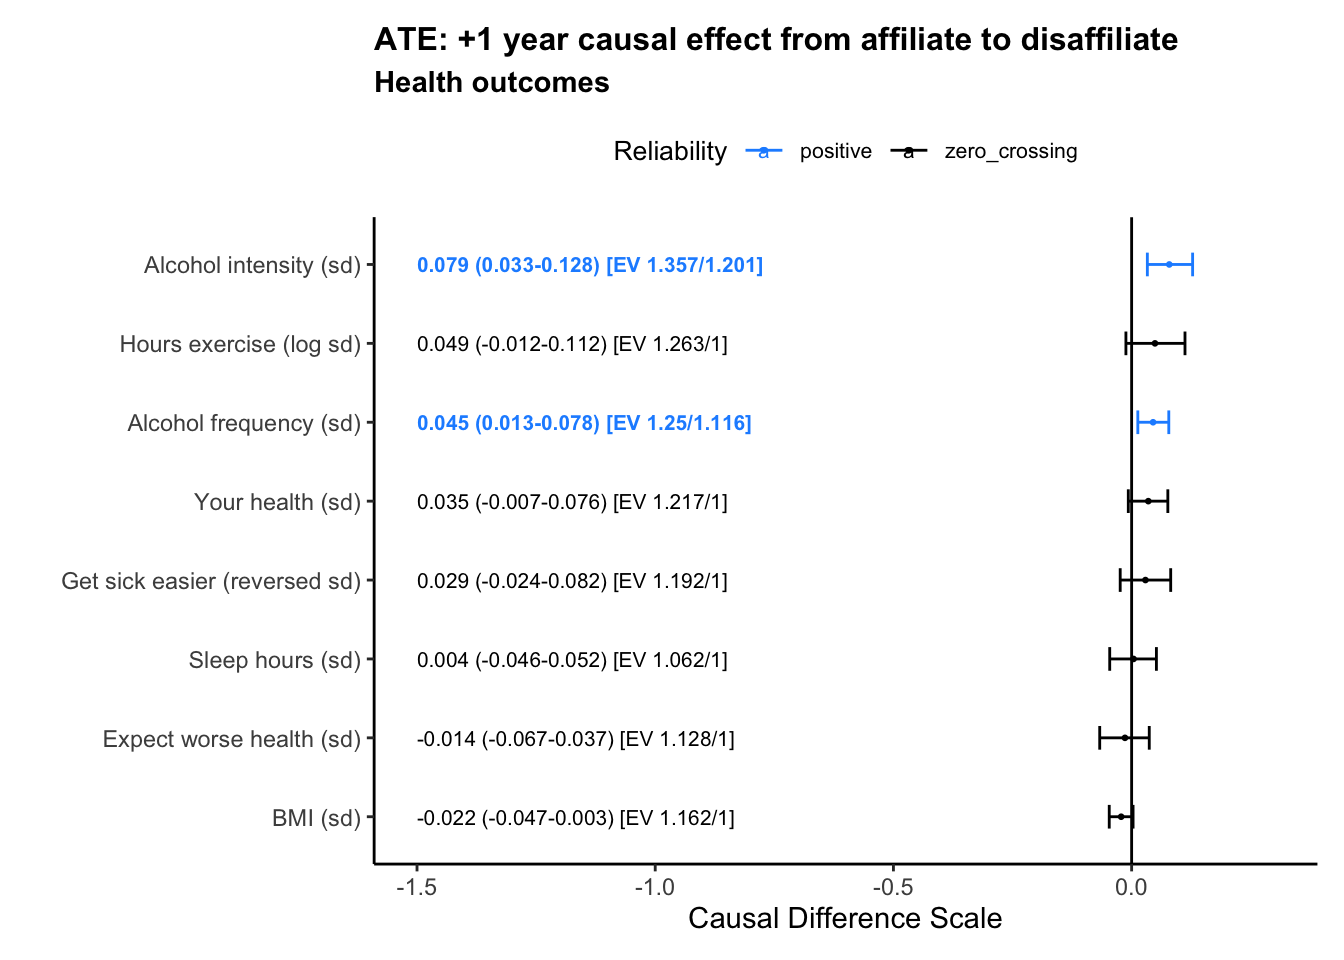
\includegraphics{ow-fl-meaning-all_files/figure-pdf/fig-results-health-1.pdf}

}

\caption{\label{fig-results-health}Causal effects of religious loss on
reported physical health}

\end{figure}

\hypertarget{tbl-results-health}{}
\begin{longtable}[]{@{}
  >{\raggedright\arraybackslash}p{(\columnwidth - 10\tabcolsep) * \real{0.3704}}
  >{\raggedleft\arraybackslash}p{(\columnwidth - 10\tabcolsep) * \real{0.1975}}
  >{\raggedleft\arraybackslash}p{(\columnwidth - 10\tabcolsep) * \real{0.0988}}
  >{\raggedleft\arraybackslash}p{(\columnwidth - 10\tabcolsep) * \real{0.0864}}
  >{\raggedleft\arraybackslash}p{(\columnwidth - 10\tabcolsep) * \real{0.0988}}
  >{\raggedleft\arraybackslash}p{(\columnwidth - 10\tabcolsep) * \real{0.1481}}@{}}
\caption{\label{tbl-results-health}Table of results for the health
domain}\tabularnewline
\toprule\noalign{}
\begin{minipage}[b]{\linewidth}\raggedright
\end{minipage} & \begin{minipage}[b]{\linewidth}\raggedleft
E{[}Y(1){]}-E{[}Y(0){]}
\end{minipage} & \begin{minipage}[b]{\linewidth}\raggedleft
2.5 \%
\end{minipage} & \begin{minipage}[b]{\linewidth}\raggedleft
97.5 \%
\end{minipage} & \begin{minipage}[b]{\linewidth}\raggedleft
E\_Value
\end{minipage} & \begin{minipage}[b]{\linewidth}\raggedleft
E\_Val\_bound
\end{minipage} \\
\midrule\noalign{}
\endfirsthead
\toprule\noalign{}
\begin{minipage}[b]{\linewidth}\raggedright
\end{minipage} & \begin{minipage}[b]{\linewidth}\raggedleft
E{[}Y(1){]}-E{[}Y(0){]}
\end{minipage} & \begin{minipage}[b]{\linewidth}\raggedleft
2.5 \%
\end{minipage} & \begin{minipage}[b]{\linewidth}\raggedleft
97.5 \%
\end{minipage} & \begin{minipage}[b]{\linewidth}\raggedleft
E\_Value
\end{minipage} & \begin{minipage}[b]{\linewidth}\raggedleft
E\_Val\_bound
\end{minipage} \\
\midrule\noalign{}
\endhead
\bottomrule\noalign{}
\endlastfoot
BMI (sd) & -0.0036 & -0.0201 & 0.0125 & 1.061 & 1.000 \\
Alcohol frequency (sd) & -0.0001 & -0.0257 & 0.0256 & 1.010 & 1.000 \\
Alcohol intensity (sd) & -0.0072 & -0.0373 & 0.0224 & 1.088 & 1.000 \\
Hours exercise (log sd) & 0.0413 & 0.0031 & 0.0760 & 1.238 & 1.072 \\
Your health (sd) & 0.1547 & 0.1248 & 0.1856 & 1.568 & 1.486 \\
Get sick easier (reversed sd) & 0.0444 & 0.0099 & 0.0773 & 1.248 &
1.110 \\
Expect worse health (sd) & 0.1094 & 0.0778 & 0.1390 & 1.445 & 1.357 \\
Sleep hours (sd) & 0.0399 & 0.0086 & 0.0696 & 1.233 & 1.102 \\
\end{longtable}

Table~\ref{tbl-results-health} presents the Population Average Treatment
Effect (PATE) which is the expected difference in outcomes between
treatment and control groups for the New Zealand population. We observed
the following:

\begin{figure}

{\centering 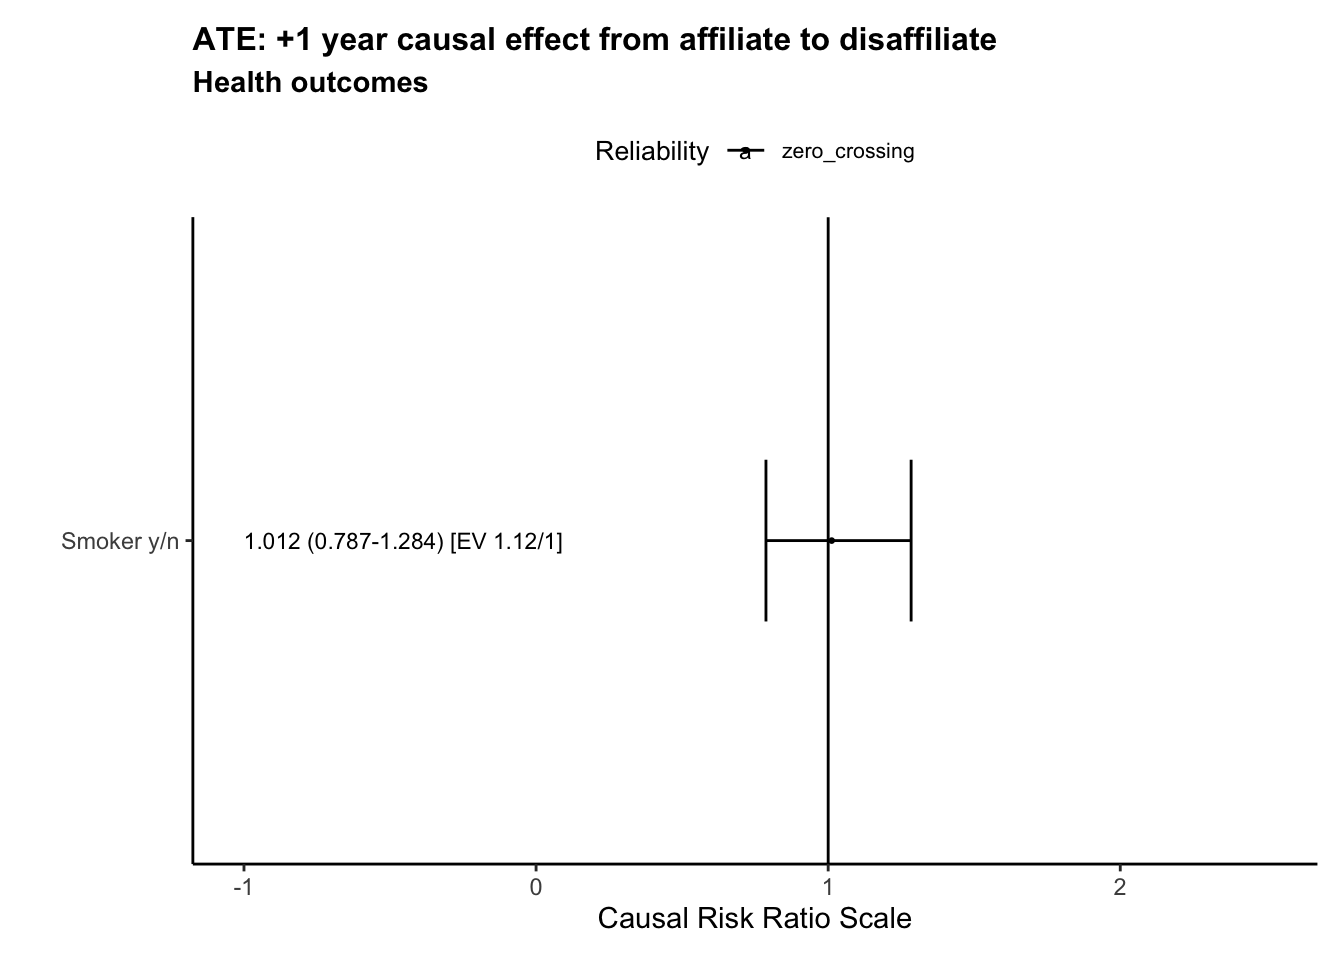
\includegraphics{ow-fl-meaning-all_files/figure-pdf/fig-results-health-rr-1.pdf}

}

\caption{\label{fig-results-health-rr}Causal effects of religious loss
on smoking (risk ratio)}

\end{figure}

\hypertarget{tbl-results-health-rr}{}
\begin{longtable}[]{@{}lrrrrr@{}}
\caption{\label{tbl-results-health-rr}Table of results for
smoking}\tabularnewline
\toprule\noalign{}
& E{[}Y(1){]}/E{[}Y(0){]} & 2.5 \% & 97.5 \% & E\_Value &
E\_Val\_bound \\
\midrule\noalign{}
\endfirsthead
\toprule\noalign{}
& E{[}Y(1){]}/E{[}Y(0){]} & 2.5 \% & 97.5 \% & E\_Value &
E\_Val\_bound \\
\midrule\noalign{}
\endhead
\bottomrule\noalign{}
\endlastfoot
Smoker y/n & 0.9992 & 0.8504 & 1.1851 & 1.029 & 1 \\
\end{longtable}

For the outcome `Smoker y/n', the PATE causal contrast is XXX. The
confidence interval ranges from XXX to XXX The E-value for this outcome
confirms the causal contrast unreliable.

\hypertarget{effects-on-embodied-well-being-first-to-third-quartile-intevention-on-meaning-of-life}{%
\subsection{Effects on embodied well-being (first to third quartile
intevention on meaning of
life)}\label{effects-on-embodied-well-being-first-to-third-quartile-intevention-on-meaning-of-life}}

\begin{figure}

{\centering 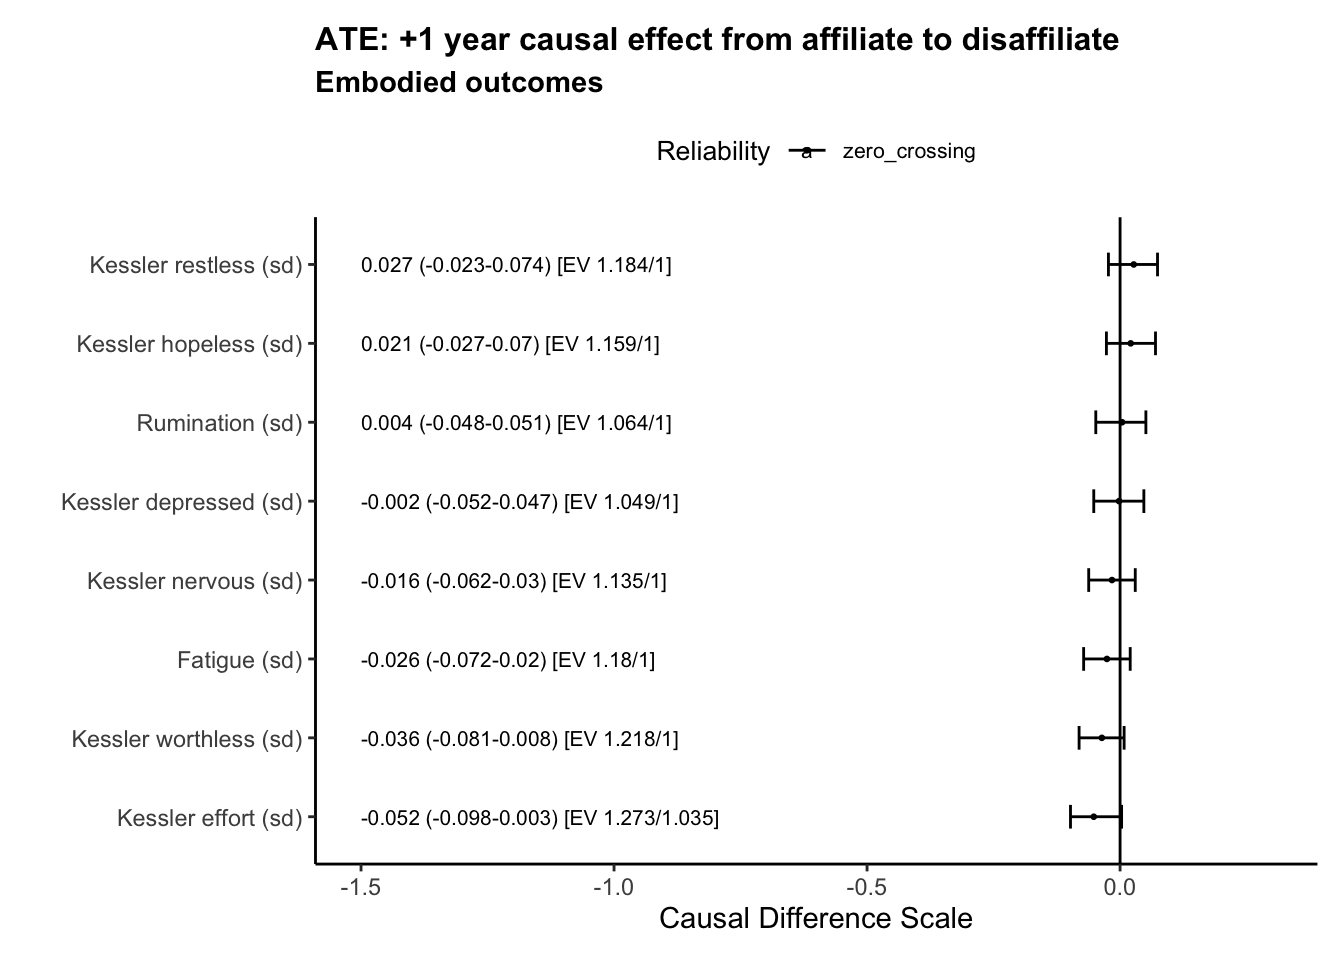
\includegraphics{ow-fl-meaning-all_files/figure-pdf/fig-results-embodied-1.pdf}

}

\caption{\label{fig-results-embodied}Causal effects of religious loss on
embodied well-being}

\end{figure}

\hypertarget{tbl-results-embodied}{}
\begin{longtable}[]{@{}
  >{\raggedright\arraybackslash}p{(\columnwidth - 10\tabcolsep) * \real{0.3067}}
  >{\raggedleft\arraybackslash}p{(\columnwidth - 10\tabcolsep) * \real{0.2133}}
  >{\raggedleft\arraybackslash}p{(\columnwidth - 10\tabcolsep) * \real{0.1067}}
  >{\raggedleft\arraybackslash}p{(\columnwidth - 10\tabcolsep) * \real{0.1067}}
  >{\raggedleft\arraybackslash}p{(\columnwidth - 10\tabcolsep) * \real{0.1067}}
  >{\raggedleft\arraybackslash}p{(\columnwidth - 10\tabcolsep) * \real{0.1600}}@{}}
\caption{\label{tbl-results-embodied}Table of results for the embodied
well-being domain}\tabularnewline
\toprule\noalign{}
\begin{minipage}[b]{\linewidth}\raggedright
\end{minipage} & \begin{minipage}[b]{\linewidth}\raggedleft
E{[}Y(1){]}-E{[}Y(0){]}
\end{minipage} & \begin{minipage}[b]{\linewidth}\raggedleft
2.5 \%
\end{minipage} & \begin{minipage}[b]{\linewidth}\raggedleft
97.5 \%
\end{minipage} & \begin{minipage}[b]{\linewidth}\raggedleft
E\_Value
\end{minipage} & \begin{minipage}[b]{\linewidth}\raggedleft
E\_Val\_bound
\end{minipage} \\
\midrule\noalign{}
\endfirsthead
\toprule\noalign{}
\begin{minipage}[b]{\linewidth}\raggedright
\end{minipage} & \begin{minipage}[b]{\linewidth}\raggedleft
E{[}Y(1){]}-E{[}Y(0){]}
\end{minipage} & \begin{minipage}[b]{\linewidth}\raggedleft
2.5 \%
\end{minipage} & \begin{minipage}[b]{\linewidth}\raggedleft
97.5 \%
\end{minipage} & \begin{minipage}[b]{\linewidth}\raggedleft
E\_Value
\end{minipage} & \begin{minipage}[b]{\linewidth}\raggedleft
E\_Val\_bound
\end{minipage} \\
\midrule\noalign{}
\endhead
\bottomrule\noalign{}
\endlastfoot
Fatigue (sd) & -0.1059 & -0.1384 & -0.0723 & 1.435 & 1.339 \\
Rumination (sd) & -0.1993 & -0.2327 & -0.1643 & 1.687 & 1.596 \\
Kessler depressed (sd) & -0.2061 & -0.2408 & -0.1715 & 1.705 & 1.613 \\
Kessler effort (sd) & -0.1462 & -0.1788 & -0.1145 & 1.545 & 1.458 \\
Kessler hopeless (sd) & -0.2426 & -0.2797 & -0.2096 & 1.802 & 1.709 \\
Kessler nervous (sd) & -0.1199 & -0.1526 & -0.0883 & 1.474 & 1.383 \\
Kessler restless (sd) & -0.1003 & -0.1331 & -0.0687 & 1.419 & 1.325 \\
Kessler worthless (sd) & -0.2422 & -0.2732 & -0.2102 & 1.801 & 1.718 \\
\end{longtable}

Table~\ref{tbl-results-embodied} presents the Population Average
Treatment Effect (PATE) for the embodied domain.

\hypertarget{effects-on-practical-well-being-first-to-third-quartile-intevention-on-meaning-of-life}{%
\subsection{Effects on practical well-being (first to third quartile
intevention on meaning of
life)}\label{effects-on-practical-well-being-first-to-third-quartile-intevention-on-meaning-of-life}}

\begin{figure}

{\centering 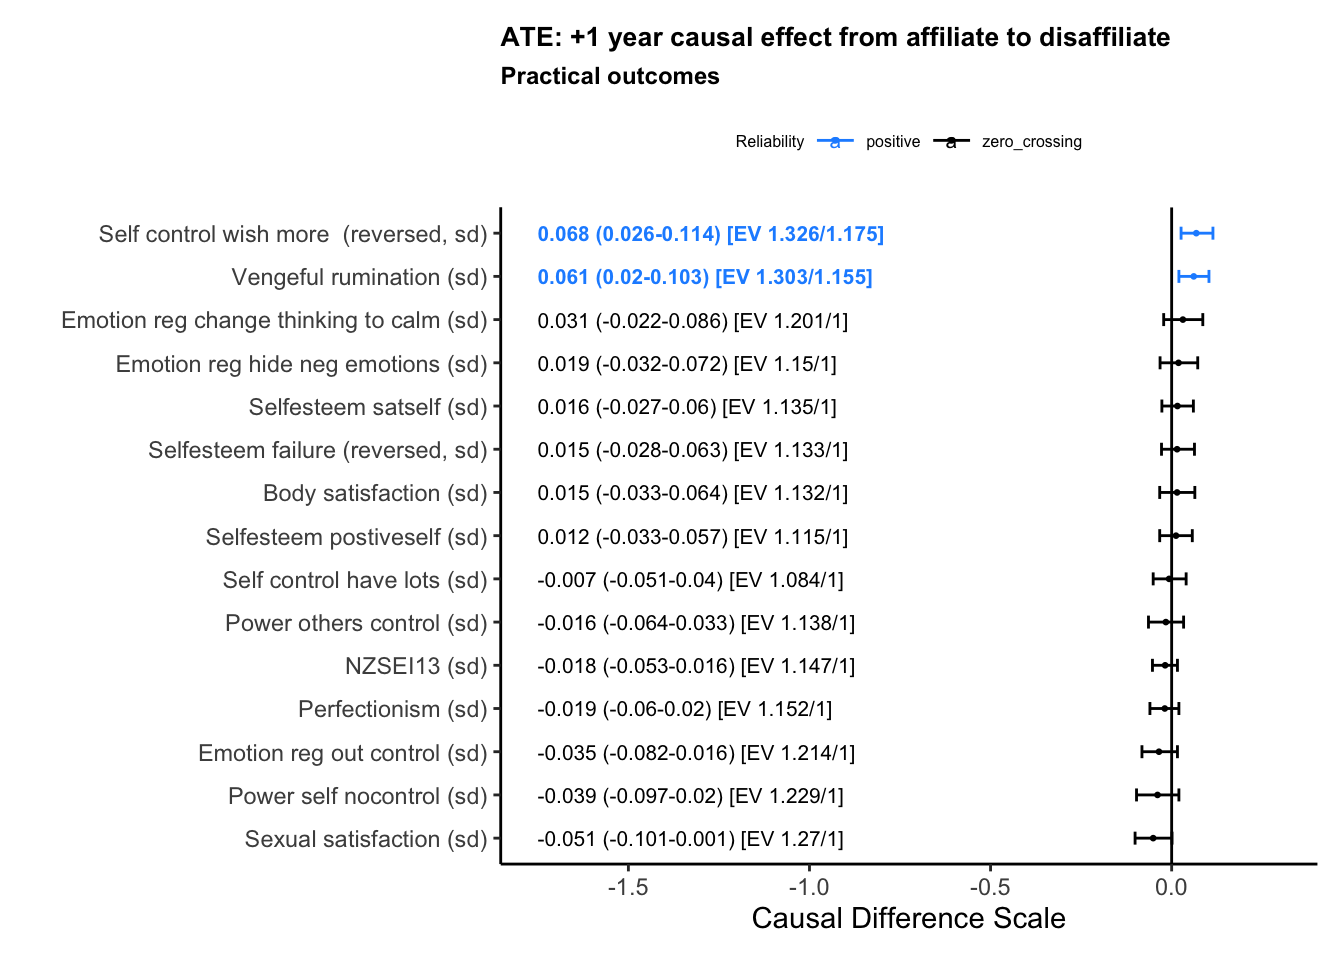
\includegraphics{ow-fl-meaning-all_files/figure-pdf/fig-results-practical-well-being-1.pdf}

}

\caption{\label{fig-results-practical-well-being}Causal effects of
religious loss on practical well-being}

\end{figure}

\hypertarget{tbl-results-practical}{}
\begin{longtable}[]{@{}
  >{\raggedright\arraybackslash}p{(\columnwidth - 10\tabcolsep) * \real{0.4409}}
  >{\raggedleft\arraybackslash}p{(\columnwidth - 10\tabcolsep) * \real{0.1720}}
  >{\raggedleft\arraybackslash}p{(\columnwidth - 10\tabcolsep) * \real{0.0860}}
  >{\raggedleft\arraybackslash}p{(\columnwidth - 10\tabcolsep) * \real{0.0860}}
  >{\raggedleft\arraybackslash}p{(\columnwidth - 10\tabcolsep) * \real{0.0860}}
  >{\raggedleft\arraybackslash}p{(\columnwidth - 10\tabcolsep) * \real{0.1290}}@{}}
\caption{\label{tbl-results-practical}Table of results for the practical
well-being domain}\tabularnewline
\toprule\noalign{}
\begin{minipage}[b]{\linewidth}\raggedright
\end{minipage} & \begin{minipage}[b]{\linewidth}\raggedleft
E{[}Y(1){]}-E{[}Y(0){]}
\end{minipage} & \begin{minipage}[b]{\linewidth}\raggedleft
2.5 \%
\end{minipage} & \begin{minipage}[b]{\linewidth}\raggedleft
97.5 \%
\end{minipage} & \begin{minipage}[b]{\linewidth}\raggedleft
E\_Value
\end{minipage} & \begin{minipage}[b]{\linewidth}\raggedleft
E\_Val\_bound
\end{minipage} \\
\midrule\noalign{}
\endfirsthead
\toprule\noalign{}
\begin{minipage}[b]{\linewidth}\raggedright
\end{minipage} & \begin{minipage}[b]{\linewidth}\raggedleft
E{[}Y(1){]}-E{[}Y(0){]}
\end{minipage} & \begin{minipage}[b]{\linewidth}\raggedleft
2.5 \%
\end{minipage} & \begin{minipage}[b]{\linewidth}\raggedleft
97.5 \%
\end{minipage} & \begin{minipage}[b]{\linewidth}\raggedleft
E\_Value
\end{minipage} & \begin{minipage}[b]{\linewidth}\raggedleft
E\_Val\_bound
\end{minipage} \\
\midrule\noalign{}
\endhead
\bottomrule\noalign{}
\endlastfoot
Sexual satisfaction (sd) & 0.1245 & 0.0910 & 0.1598 & 1.487 & 1.390 \\
Perfectionism (sd) & -0.2148 & -0.2420 & -0.1863 & 1.728 & 1.654 \\
Body satisfaction (sd) & 0.1052 & 0.0714 & 0.1378 & 1.433 & 1.337 \\
Vengeful rumination (sd) & -0.1729 & -0.2075 & -0.1376 & 1.617 &
1.523 \\
Power self nocontrol (sd) & -0.1945 & -0.2288 & -0.1577 & 1.674 &
1.580 \\
Power others control (sd) & -0.1544 & -0.1920 & -0.1173 & 1.568 &
1.466 \\
Selfesteem satself (sd) & 0.2795 & 0.2480 & 0.3105 & 1.901 & 1.817 \\
Selfesteem postiveself (sd) & 0.2474 & 0.2160 & 0.2781 & 1.815 &
1.732 \\
Selfesteem failure (reversed, sd) & 0.2063 & 0.1760 & 0.2391 & 1.706 &
1.622 \\
Self control have lots (sd) & 0.1404 & 0.1067 & 0.1749 & 1.530 &
1.436 \\
Self control wish more (reversed, sd) & 0.0935 & 0.0624 & 0.1247 & 1.400
& 1.307 \\
Emotion reg out control (sd) & -0.1447 & -0.1784 & -0.1100 & 1.541 &
1.448 \\
Emotion reg hide neg emotions (sd) & -0.0990 & -0.1311 & -0.0657 & 1.415
& 1.319 \\
Emotion reg change thinking to calm (sd) & 0.1720 & 0.1357 & 0.2091 &
1.615 & 1.516 \\
\end{longtable}

Table~\ref{tbl-results-practical}

\hypertarget{effects-on-reflective-well-being-first-to-third-quartile-intevention-on-meaning-of-life}{%
\subsection{Effects on reflective well-being (first to third quartile
intevention on meaning of
life)}\label{effects-on-reflective-well-being-first-to-third-quartile-intevention-on-meaning-of-life}}

\begin{figure}

{\centering \includegraphics{ow-fl-meaning-all_files/figure-pdf/fig-results-reflective-well-being-1.pdf}

}

\caption{\label{fig-results-reflective-well-being}Causal effects of
religious loss on reflective well-being}

\end{figure}

\hypertarget{tbl-results-reflective}{}
\begin{longtable}[]{@{}
  >{\raggedright\arraybackslash}p{(\columnwidth - 10\tabcolsep) * \real{0.3243}}
  >{\raggedleft\arraybackslash}p{(\columnwidth - 10\tabcolsep) * \real{0.2162}}
  >{\raggedleft\arraybackslash}p{(\columnwidth - 10\tabcolsep) * \real{0.0946}}
  >{\raggedleft\arraybackslash}p{(\columnwidth - 10\tabcolsep) * \real{0.0946}}
  >{\raggedleft\arraybackslash}p{(\columnwidth - 10\tabcolsep) * \real{0.1081}}
  >{\raggedleft\arraybackslash}p{(\columnwidth - 10\tabcolsep) * \real{0.1622}}@{}}
\caption{\label{tbl-results-reflective}Table of results for the
reflective well-being domain}\tabularnewline
\toprule\noalign{}
\begin{minipage}[b]{\linewidth}\raggedright
\end{minipage} & \begin{minipage}[b]{\linewidth}\raggedleft
E{[}Y(1){]}-E{[}Y(0){]}
\end{minipage} & \begin{minipage}[b]{\linewidth}\raggedleft
2.5 \%
\end{minipage} & \begin{minipage}[b]{\linewidth}\raggedleft
97.5 \%
\end{minipage} & \begin{minipage}[b]{\linewidth}\raggedleft
E\_Value
\end{minipage} & \begin{minipage}[b]{\linewidth}\raggedleft
E\_Val\_bound
\end{minipage} \\
\midrule\noalign{}
\endfirsthead
\toprule\noalign{}
\begin{minipage}[b]{\linewidth}\raggedright
\end{minipage} & \begin{minipage}[b]{\linewidth}\raggedleft
E{[}Y(1){]}-E{[}Y(0){]}
\end{minipage} & \begin{minipage}[b]{\linewidth}\raggedleft
2.5 \%
\end{minipage} & \begin{minipage}[b]{\linewidth}\raggedleft
97.5 \%
\end{minipage} & \begin{minipage}[b]{\linewidth}\raggedleft
E\_Value
\end{minipage} & \begin{minipage}[b]{\linewidth}\raggedleft
E\_Val\_bound
\end{minipage} \\
\midrule\noalign{}
\endhead
\bottomrule\noalign{}
\endlastfoot
Gratitude (sd) & 0.2792 & 0.2481 & 0.3122 & 1.900 & 1.814 \\
Pwi health (sd) & 0.1478 & 0.1146 & 0.1816 & 1.550 & 1.459 \\
Pwi relationships (sd) & 0.2045 & 0.1691 & 0.2393 & 1.701 & 1.608 \\
Pwi security (sd) & 0.1560 & 0.1161 & 0.1904 & 1.572 & 1.471 \\
Pwi standardliving (sd) & 0.1209 & 0.0869 & 0.1544 & 1.477 & 1.382 \\
Lifesat satlife (sd) & 0.2994 & 0.2639 & 0.3341 & 1.954 & 1.860 \\
Lifesat ideal (sd) & 0.2553 & 0.2231 & 0.2891 & 1.836 & 1.748 \\
\end{longtable}

Table~\ref{tbl-results-reflective}

\hypertarget{effects-social-well-being-first-to-third-quartile-intevention-on-meaning-of-life}{%
\subsection{Effects social well-being (first to third quartile
intevention on meaning of
life)}\label{effects-social-well-being-first-to-third-quartile-intevention-on-meaning-of-life}}

\begin{figure}

{\centering \includegraphics{ow-fl-meaning-all_files/figure-pdf/fig-results-social-wellbeing-1.pdf}

}

\caption{\label{fig-results-social-wellbeing}Causal effects of religious
loss on social well-being}

\end{figure}

\hypertarget{tbl-results-social}{}
\begin{longtable}[]{@{}
  >{\raggedright\arraybackslash}p{(\columnwidth - 10\tabcolsep) * \real{0.3243}}
  >{\raggedleft\arraybackslash}p{(\columnwidth - 10\tabcolsep) * \real{0.2162}}
  >{\raggedleft\arraybackslash}p{(\columnwidth - 10\tabcolsep) * \real{0.0946}}
  >{\raggedleft\arraybackslash}p{(\columnwidth - 10\tabcolsep) * \real{0.0946}}
  >{\raggedleft\arraybackslash}p{(\columnwidth - 10\tabcolsep) * \real{0.1081}}
  >{\raggedleft\arraybackslash}p{(\columnwidth - 10\tabcolsep) * \real{0.1622}}@{}}
\caption{\label{tbl-results-social}Table of results for the reflective
well-being domain}\tabularnewline
\toprule\noalign{}
\begin{minipage}[b]{\linewidth}\raggedright
\end{minipage} & \begin{minipage}[b]{\linewidth}\raggedleft
E{[}Y(1){]}-E{[}Y(0){]}
\end{minipage} & \begin{minipage}[b]{\linewidth}\raggedleft
2.5 \%
\end{minipage} & \begin{minipage}[b]{\linewidth}\raggedleft
97.5 \%
\end{minipage} & \begin{minipage}[b]{\linewidth}\raggedleft
E\_Value
\end{minipage} & \begin{minipage}[b]{\linewidth}\raggedleft
E\_Val\_bound
\end{minipage} \\
\midrule\noalign{}
\endfirsthead
\toprule\noalign{}
\begin{minipage}[b]{\linewidth}\raggedright
\end{minipage} & \begin{minipage}[b]{\linewidth}\raggedleft
E{[}Y(1){]}-E{[}Y(0){]}
\end{minipage} & \begin{minipage}[b]{\linewidth}\raggedleft
2.5 \%
\end{minipage} & \begin{minipage}[b]{\linewidth}\raggedleft
97.5 \%
\end{minipage} & \begin{minipage}[b]{\linewidth}\raggedleft
E\_Value
\end{minipage} & \begin{minipage}[b]{\linewidth}\raggedleft
E\_Val\_bound
\end{minipage} \\
\midrule\noalign{}
\endhead
\bottomrule\noalign{}
\endlastfoot
Gratitude (sd) & 0.2792 & 0.2481 & 0.3122 & 1.900 & 1.814 \\
Pwi health (sd) & 0.1478 & 0.1146 & 0.1816 & 1.550 & 1.459 \\
Pwi relationships (sd) & 0.2045 & 0.1691 & 0.2393 & 1.701 & 1.608 \\
Pwi security (sd) & 0.1560 & 0.1161 & 0.1904 & 1.572 & 1.471 \\
Pwi standardliving (sd) & 0.1209 & 0.0869 & 0.1544 & 1.477 & 1.382 \\
Lifesat satlife (sd) & 0.2994 & 0.2639 & 0.3341 & 1.954 & 1.860 \\
Lifesat ideal (sd) & 0.2553 & 0.2231 & 0.2891 & 1.836 & 1.748 \\
\end{longtable}

Table~\ref{tbl-results-social}

\hypertarget{discussion}{%
\section{Discussion}\label{discussion}}

Here, we combined rigorous methods from causal epidemiology with
national scale time-series data to estimate the causal effects of
meaning of life on multidimensional well-being. We used doubly robust
methods that combine propensity score weights with regression
stratification. By controlling for measures of all outcomes at baseline
we reduce the probability of unmeasured confounding. Because this cannot
be ensured, we report E-values, a sensitivity analysis that clarifies
the ``worst case'' scenario for an unmeasured confounder to explain away
the results.

\textbf{Health domain}: The expected +1 year effect\ldots{}

Note it is interesting that meaning of life should be causally
associated with increasing belief that I will get sick. This suggests
(realism?)

\textbf{Embodied well-being domains}:The expected +1 year effect\ldots{}

\textbf{Practical well-being}: The expected +1 year effect\ldots{}

\textbf{Reflective well-being}: The expected +1 year effect \ldots{}

\textbf{Social well-being-being}: The expected +1 year effect \ldots{}

\hypertarget{generalisability-and-transportability}{%
\subsection{Generalisability and
Transportability}\label{generalisability-and-transportability}}

\hypertarget{assumptions-and-limitations}{%
\subsection{Assumptions and
Limitations}\label{assumptions-and-limitations}}

\hypertarget{theoretical-relevance}{%
\subsection{Theoretical Relevance}\label{theoretical-relevance}}

This study is important both for its methods and findings.

\begin{enumerate}
\def\labelenumi{\arabic{enumi}.}
\tightlist
\item
  The bar for causality in this study very high\ldots{}
\end{enumerate}

\hypertarget{future-research}{%
\subsection{Future Research}\label{future-research}}

\hypertarget{real-world-implications}{%
\subsection{Real-world Implications}\label{real-world-implications}}

\hypertarget{ethics-approval-details}{%
\subsection{Ethics Approval Details}\label{ethics-approval-details}}

The NZAVS is reviewed every three years by the University of Auckland
Human Participants Ethics Committee. Our most recent ethics approval
statement is as follows: The New Zealand Attitudes and Values Study was
approved by the University of Auckland Human Participants Ethics
Committee on 26/05/2021 for six years until 26/05/2027, Reference Number
UAHPEC22576.

\hypertarget{acknowledgements}{%
\subsection{Acknowledgements}\label{acknowledgements}}

The New Zealand Attitudes and Values Study is supported by a grant from
the TempletoReligion Trust (TRT0196; TRT0418). JB received support from
the Max Planck Institute for the Science of Human History. The funders
had no role in preparing the manuscript or the decision to publish.

\newpage{}

\hypertarget{appendix-a.-measures}{%
\section{Appendix A. Measures}\label{appendix-a.-measures}}

\hypertarget{baseline-confounding-control}{%
\subsection{Baseline confounding
control}\label{baseline-confounding-control}}

\hypertarget{age-waves-1-15}{%
\subsubsection{Age (waves: 1-15)}\label{age-waves-1-15}}

We asked participants' age in an open-ended question (``What is your
age?'' or ``What is your date of birth'').

\hypertarget{disability-waves-5-15}{%
\subsubsection{Disability (waves: 5-15)}\label{disability-waves-5-15}}

We assessed disability with a one item indicator adapted from Verbrugge
(\protect\hyperlink{ref-verbrugge1997}{1997}), that asks ``Do you have a
health condition or disability that limits you, and that has lasted for
6+ months?'' (1 = Yes, 0 = No).

\hypertarget{education-attainment-waves-1-4-15}{%
\subsubsection{Education Attainment (waves: 1,
4-15)}\label{education-attainment-waves-1-4-15}}

Participants were asked ``What is your highest level of
qualification?''. We coded participans highest finished degree according
to the New Zealand Qualifications Authority. Ordinal-Rank 0-10 NZREG
codes (with overseas school quals coded as Level 3, and all other
ancillary categories coded as missing)
See:https://www.nzqa.govt.nz/assets/Studying-in-NZ/New-Zealand-Qualification-Framework/requirements-nzqf.pdf

\hypertarget{employment-waves-1-3-4-11}{%
\subsubsection{Employment (waves: 1-3,
4-11)}\label{employment-waves-1-3-4-11}}

We asked participants ``Are you currently employed? (This includes
self-employed or casual work)''. * note: This question disappeared in
the updated NZAVS Technical documents (Data Dictionary).

\hypertarget{european-waves-1-15}{%
\subsubsection{European (waves: 1-15)}\label{european-waves-1-15}}

Participants were asked ``Which ethnic group do you belong to (NZ census
question)?'' or ``Which ethnic group(s) do you belong to? (Open-ended)''
(wave: 3). Europeans were coded as 1, whereas other ethnicities were
coded as 0.

\hypertarget{ethnicity-waves-3}{%
\subsubsection{Ethnicity (waves: 3)}\label{ethnicity-waves-3}}

Based on the New Zealand Cencus, we asked participants ``Which ethnic
group(s) do you belong to?''. The responses were: (1) New Zealand
European; (2) Māori; (3) Samoan; (4) Cook Island Māori; (5) Tongan; (6)
Niuean; (7) Chinese; (8) Indian; (9) Other such as DUTCH, JAPANESE,
TOKELAUAN. Please state:. We coded their answers into four groups:
Maori, Pacific, Asian, and Euro (except for Time 3, which used an
open-ended measure).

\hypertarget{gender-waves-1-15}{%
\subsubsection{Gender (waves: 1-15)}\label{gender-waves-1-15}}

We asked participants' gender in an open-ended question: ``what is your
gender?'' or ``Are you male or female?'' (waves: 1-5). Female was coded
as 0, Male was coded as 1, and gender diverse coded as 3
(\protect\hyperlink{ref-fraser_coding_2020}{Fraser et al. 2020}). (or
0.5 = neither female nor male)

\hypertarget{income-waves-1-3-4-15}{%
\subsubsection{Income (waves: 1-3, 4-15)}\label{income-waves-1-3-4-15}}

Participants were asked ``Please estimate your total household income
(before tax) for the year XXXX''. To stablise this indicator, we first
took the natural log of the response + 1, and then centred and
standardised the log-transformed indicator.

\hypertarget{number-of-children-waves-1-3-4-15}{%
\subsubsection{Number of Children (waves: 1-3,
4-15)}\label{number-of-children-waves-1-3-4-15}}

We measured number of children using one item from Bulbulia
(\protect\hyperlink{ref-Bulbulia_2015}{2015}). We asked participants
``How many children have you given birth to, fathered, or adopted. How
many children have you given birth to, fathered, or adopted?'' or
````How many children have you given birth to, fathered, or adopted. How
many children have you given birth to, fathered, and/or parented?''
(waves: 12-15).

\hypertarget{political-orientation}{%
\subsubsection{Political Orientation}\label{political-orientation}}

We measured participants' political orientation using a single item
adapted from Jost (\protect\hyperlink{ref-jost_end_2006-1}{2006}).

``Please rate how politically liberal versus conservative you see
yourself as being.''

(1 = Extremely Liberal to 7 = Extremely Conservative)

\hypertarget{nzsei-13-waves-8-15}{%
\subsubsection{NZSEI-13 (waves: 8-15)}\label{nzsei-13-waves-8-15}}

We assessed occupational prestige and status using the New Zealand
Socio-economic Index 13 (NZSEI-13)
(\protect\hyperlink{ref-fahy2017}{Fahy, Lee, and Milne 2017}). This
index uses the income, age, and education of a reference group, in this
case the 2013 New Zealand census, to calculate an score for each
occupational group. Scores range from 10 (Lowest) to 90 (Highest). This
list of index scores for occupational groups was used to assign each
participant a NZSEI-13 score based on their occupation.

Participants were asked ``If you are a parent, what is the birth date of
your eldest child?''.

\hypertarget{living-with-partner}{%
\subsubsection{Living with Partner}\label{living-with-partner}}

Participants were asekd ``Do you live with your partner?'' (1 = Yes, 0 =
No).

\hypertarget{living-in-an-urban-area-waves-1-15}{%
\subsubsection{Living in an Urban Area (waves:
1-15)}\label{living-in-an-urban-area-waves-1-15}}

We coded whether they are living in an urban or rural area (1 = Urban, 0
= Rural) based on the addresses provided.

We coded whether they are living in an urban or rural area (1 = Urban, 0
= Rural) based on the addresses provided.

\hypertarget{nz-deprivation-index-waves-1-15}{%
\subsubsection{NZ Deprivation Index (waves:
1-15)}\label{nz-deprivation-index-waves-1-15}}

We used the NZ Deprivation Index to assign each participant a score
based on where they live (\protect\hyperlink{ref-atkinson2019}{Atkinson,
Salmond, and Crampton 2019}). This score combines data such as income,
home ownership, employment, qualifications, family structure, housing,
and access to transport and communication for an area into one
deprivation score.

\hypertarget{nz-born-waves-1-24-15}{%
\subsubsection{NZ-Born (waves: 1-2,4-15)}\label{nz-born-waves-1-24-15}}

We asked participants ``Which country were you born in?'' or ``Where
were you born? (please be specific, e.g., which town/city?)'' (waves:
6-15).

\hypertarget{mini-ipip-6-waves-1-34-15}{%
\subsubsection{Mini-IPIP 6 (waves:
1-3,4-15)}\label{mini-ipip-6-waves-1-34-15}}

We measured participants personality with the Mini International
Personality Item Pool 6 (Mini-IPIP6)
(\protect\hyperlink{ref-sibley2011}{Chris G. Sibley et al. 2011}) which
consists of six dimensions and each dimensions is measured with four
items:

\begin{enumerate}
\def\labelenumi{\arabic{enumi}.}
\item
  agreeableness,

  \begin{enumerate}
  \def\labelenumii{\roman{enumii}.}
  \tightlist
  \item
    I sympathize with others' feelings.
  \item
    I am not interested in other people's problems. (r)
  \item
    I feel others' emotions.
  \item
    I am not really interested in others. (r)
  \end{enumerate}
\item
  conscientiousness,

  \begin{enumerate}
  \def\labelenumii{\roman{enumii}.}
  \tightlist
  \item
    I get chores done right away.
  \item
    I like order.
  \item
    I make a mess of things. (r)
  \item
    I ften forget to put things back in their proper place. (r)
  \end{enumerate}
\item
  extraversion,

  \begin{enumerate}
  \def\labelenumii{\roman{enumii}.}
  \tightlist
  \item
    I am the life of the party.
  \item
    I don't talk a lot. (r)
  \item
    I keep in the background. (r)
  \item
    I talk to a lot of different people at parties.
  \end{enumerate}
\item
  honesty-humility,

  \begin{enumerate}
  \def\labelenumii{\roman{enumii}.}
  \tightlist
  \item
    I feel entitled to more of everything. (r)
  \item
    I deserve more things in life. (r)
  \item
    I would like to be seen driving around in a very expensive car. (r)
  \item
    I would get a lot of pleasure from owning expensive luxury goods.
    (r)
  \end{enumerate}
\item
  neuroticism, and

  \begin{enumerate}
  \def\labelenumii{\roman{enumii}.}
  \tightlist
  \item
    I have frequent mood swings.
  \item
    I am relaxed most of the time. (r)
  \item
    I get upset easily.
  \item
    I seldom feel blue. (r)
  \end{enumerate}
\item
  openness to experience

  \begin{enumerate}
  \def\labelenumii{\roman{enumii}.}
  \tightlist
  \item
    I have a vivid imagination.
  \item
    I have difficulty understanding abstract ideas. (r)
  \item
    I do not have a good imagination. (r)
  \item
    I am not interested in abstract ideas. (r)
  \end{enumerate}
\end{enumerate}

Each dimension was assessed with four items and participants rated the
accuracy of each item as it applies to them from 1 (Very Inaccurate) to
7 (Very Accurate). Items marked with (r) are reverse coded.

\hypertarget{honesty-humility-modesty-facet-waves-10-14}{%
\subsubsection{Honesty-Humility-Modesty Facet (waves:
10-14)}\label{honesty-humility-modesty-facet-waves-10-14}}

Participants indicated the extent to which they agree with the following
four statements from Campbell et al.
(\protect\hyperlink{ref-campbell2004}{2004}) , and Chris G. Sibley et
al. (\protect\hyperlink{ref-sibley2011}{2011}) (1 = Strongly Disagree to
7 = Strongly Agree)

\begin{verbatim}
i.  I want people to know that I am an important person of high status, (Waves: 1, 10-14)
ii. I am an ordinary person who is no better than others.
iii. I wouldn't want people to treat me as though I were superior to them.
iv. I think that I am entitled to more respect than the average person is.
\end{verbatim}

\hypertarget{exposure-variable}{%
\subsection{Exposure variable}\label{exposure-variable}}

\hypertarget{meaning-of-life-waves-10-15}{%
\subsubsection{Meaning of Life (waves:
10-15)}\label{meaning-of-life-waves-10-15}}

We assessed participants' levels of life meaning using two items from
Steger et al. (\protect\hyperlink{ref-steger_meaning_2006}{2006}):

\begin{verbatim}
1.  My life has a clear sense of purpose;
2.  I have a good sense of what makes my life meaningful.
\end{verbatim}

Participants indicated their agreement with these items (1 = Strongly
Disagree to 7 = Strongly Agree).

\hypertarget{health-well-being-outcomes}{%
\subsection{Health well-being
outcomes}\label{health-well-being-outcomes}}

\hypertarget{alcohol-frequency-waves-6-15}{%
\subsubsection{Alcohol Frequency (waves:
6-15)}\label{alcohol-frequency-waves-6-15}}

We measured participants' frequency of drinking alcohol using one item
adapted from Health
(\protect\hyperlink{ref-Ministry_of_Health_2013}{2013}) . Participants
were asked ``How often do you have a drink containing alcohol?'' (1 =
Never - I don't drink, 2 = Monthly or less, 3 = Up to 4 times a month, 4
= Up to 3 times a week, 5 = 4 or more times a week, 6 = Don't know).

\hypertarget{alcohol-intensity-waves-6-15}{%
\subsubsection{Alcohol Intensity (waves:
6-15)}\label{alcohol-intensity-waves-6-15}}

We measured participants' intensity of drinking alcohol using one item
adapted from (\protect\hyperlink{ref-Ministry_of_Health_2013}{Health
2013}). Participants were asked ``How many drinks containing alcohol do
you have on a typical day when drinking alcohol? (number of drinks on a
typical day when drinking)''

\hypertarget{body-mass-index-waves-2-3-4-15}{%
\subsubsection{Body Mass Index (waves: 2-3,
4-15)}\label{body-mass-index-waves-2-3-4-15}}

Participants were asked ``What is your height? (metres)'' and ``What is
your weight? (kg)''. Based on participants indication of their height
and weight we calculated the BMI by dividing the weight in kilograms by
the square of the height in meters.

\hypertarget{short-form-subjective-health-waves-5-15}{%
\subsubsection{Short-Form Subjective Health (waves:
5-15)}\label{short-form-subjective-health-waves-5-15}}

Participants' subjective health was assessed by three items selected
from the MOS 36-item short-form health survey
(\protect\hyperlink{ref-warejr1992}{Ware Jr and Sherbourne 1992}). The
items were

\begin{verbatim}
1.  "In general, would you say your health is...";
2.  "I seem to get sick a little easier than most people.";
3.  "I expect my health to get worse." Participants responded to those items on a scale (1 = Poor to 7 = Excellent).
\end{verbatim}

The second and third items were negatively-worded, so we reversed the
responses.

\hypertarget{hours-of-exercise-waves-1-4-15}{%
\subsubsection{Hours of Exercise (waves: 1,
4-15)}\label{hours-of-exercise-waves-1-4-15}}

We measured hours of exercising using one item from Chris G. Sibley et
al. (\protect\hyperlink{ref-sibley2011}{2011}). We asked participants to
estimate and report how many hours they spend in exercise/physical
activity last week. To stablise this indicator, we first took the
natural log of the response + 1, and then centred and standardised the
log-transformed indicator.

\hypertarget{hours-of-sleep-waves-5-15}{%
\subsubsection{Hours of Sleep (waves:
5-15)}\label{hours-of-sleep-waves-5-15}}

Participants were asked ``During the past month, on average, how many
hours of \emph{actual sleep} did you get per night''.

\hypertarget{smoker-waves-4-15}{%
\subsubsection{Smoker (waves: 4-15)}\label{smoker-waves-4-15}}

We asked participants whether they are currently smoking or not (1 = Yes
or 0 = No), using a single item: ``Do you currently smoke?'' or ``Do you
currently smoke tobacco cigarettes?'' (waves: 10-15) from Muriwai,
Houkamau, and Sibley
(\protect\hyperlink{ref-muriwai_looking_2018}{2018}).

\hypertarget{embodied-well-being-outcomes}{%
\subsection{Embodied well-being
outcomes}\label{embodied-well-being-outcomes}}

\hypertarget{kessler-6-waves-2-34-15}{%
\subsubsection{Kessler-6 (waves:
2-3,4-15)}\label{kessler-6-waves-2-34-15}}

We measured psychological distress using the Kessler-6 scale
(\protect\hyperlink{ref-kessler2002}{R. ~C. Kessler et al. 2002}), which
exhibits strong diagnostic concordance for moderate and severe
psychological distress in large, cross-cultural samples
(\protect\hyperlink{ref-kessler2010}{R. C. Kessler et al. 2010};
\protect\hyperlink{ref-prochaska2012}{Prochaska et al. 2012}).
Participants rated during the past 30 days, how often did\ldots{} (

\begin{verbatim}
1.  "... you feel hopeless";
2.  "... you feel so depressed that nothing could cheer you up";
3.  "... you feel restless or fidgety";
4.  "... you feel that everything was an effort";
5.  "... you feel worthless";
6.  " you feel nervous?"
\end{verbatim}

Ordinal response options for the Kessler-6 are: ``None of the time'';
``A little of the time''; ``Some of the time''; ``Most of the time'';
``All of the time.''

\hypertarget{fatigue-waves-5-15}{%
\subsubsection{Fatigue (waves: 5-15)}\label{fatigue-waves-5-15}}

We assessed subjective fatigue by asking participants, ``During the last
30 days, how often did \ldots{} you feel exhausted?'' Responses were
collected on an ordinal scale (0 = None of The Time, 1 = A little of The
Time, 2 = Some of The Time, 3 = Most of The Time, 4 = All of The Time).

\hypertarget{rumination}{%
\subsubsection{Rumination}\label{rumination}}

``During the last 30 days, how often did\ldots. you have negative
thoughts that repeated over and over?''

Ordinal response options for the Kessler-6 are: ``None of the time'';
``A little of the time''; ``Some of the time''; ``Most of the time'';
``All of the time.''

\hypertarget{practical-well-being-outcomes}{%
\subsection{Practical well-being
outcomes}\label{practical-well-being-outcomes}}

\hypertarget{body-satisfaction-waves-2-3-4-15}{%
\subsubsection{Body Satisfaction (waves: 2-3,
4-15)}\label{body-satisfaction-waves-2-3-4-15}}

We measured body satisfaction with one item from Stronge et al.
(\protect\hyperlink{ref-stronge_facebook_2015}{2015}): ``I am satisfied
with the appearance, size and shape of my body'', which participants
rated from 1 (very inaccurate) to 7 (very accurate).

\hypertarget{emotional-regulation-waves-10-13}{%
\subsubsection{Emotional Regulation (waves:
10-13)}\label{emotional-regulation-waves-10-13}}

We measured participants' levels of emotional regulation using three
items adpated from Gratz and Roemer
(\protect\hyperlink{ref-gratz_multidimensional_2004}{2004}) and Gross
and John (\protect\hyperlink{ref-gross_individual_2003}{2003}):

\begin{verbatim}
1.  "When I feel negative emotions, my emotions feel out of control.";
2.  "When I feel negative emotions, I suppress or hide my emotions.";
3.  "When I feel negative emotions, I change the way I think to help me stay calm."
\end{verbatim}

Participants were asked to indicate the extent to which they agree with
these items (1 = Strongly Disagree to 7 = Strongly Agree).

\hypertarget{perfectionism-waves-10-15}{%
\subsubsection{Perfectionism (waves:
10-15)}\label{perfectionism-waves-10-15}}

We assessed participants' perfectionism using three items from Rice,
Richardson, and Tueller (\protect\hyperlink{ref-rice_short_2014}{2014}):
(1) Doing my best never seems to be enough; (2) My performance rarely
measures up to my standards; (3) I am hardly ever satisfied with my
performance. Participants indicated the extent to which they agree with
these items (1 = Strongly Disagree to 7 = Strongly Agree).

\hypertarget{power-dependence}{%
\subsubsection{Power Dependence}\label{power-dependence}}

Participants' Power dependence was measured using two items:

\begin{verbatim}
1." I do not have enough power or control over important parts of my life."
2". Other people have too much power or control over important parts of my life. 
\end{verbatim}

Participants indicated their agreement with these items'' (1 = Strongly
Disagree to 7 = Strongly Agree).

\hypertarget{self-control-waves-5-15}{%
\subsubsection{Self-Control (waves:
5-15)}\label{self-control-waves-5-15}}

Participants were asked to indicate the extent to which they endorse the
two items

\begin{verbatim}
1.  "In general, I have a lot of self-control"
2.  "I wish I had more self-discipline"
\end{verbatim}

The scale is from Tangney, Baumeister, and Boone
(\protect\hyperlink{ref-tangney_high_2004}{2004}). The responses to the
items ranged from 1 (Strongly Disagree) to 7 (Strongly Agree).

\hypertarget{self-esteem-waves-1-3-4-15}{%
\subsubsection{Self-Esteem (waves: 1-3,
4-15)}\label{self-esteem-waves-1-3-4-15}}

We measured participants' self-esteem using three items adapted from
Rosenberg (\protect\hyperlink{ref-Rosenberg1965}{1965}). Participants
were instructed to circle the number that best represents how accurately
each statement describes them. Participants responded to the items

\begin{verbatim}
1.  "On the whole am satisfied with myself"
2.  "Take a positive attitude toward myself"
3.  "Am inclined to feel that I am a failure") on a likert-type scale (1 = Very inaccurate to 7 = Very accurate).
\end{verbatim}

\hypertarget{sexual-satisfaction-waves-10-15}{%
\subsubsection{Sexual Satisfaction (waves:
10-15)}\label{sexual-satisfaction-waves-10-15}}

Participants were asked ``How satisfied are you with your sex life?'' (1
= Not satisfied to 7 = Very satisfied).

\hypertarget{vengeful-rumination-waves-10-15}{%
\subsubsection{Vengeful Rumination (waves:
10-15)}\label{vengeful-rumination-waves-10-15}}

We assessed participants' vengeful rumination using three items,
respectively adapted from Caprara
(\protect\hyperlink{ref-caprara_indicators_1986}{1986}) and Berry et al.
(\protect\hyperlink{ref-berry_forgivingness_2005}{2005}), and developed
for NZAVS: (1) Sometimes I can't sleep because of thinking about past
wrongs I have suffered; (2) I can usually forgive and forget when
someone does me wrong; (3) I find myself regularly thinking about past
times that I have been wronged. Participants indicated their agreement
with these items (1 = Strongly Disagree to 7 = Strongly Agree). The
values for the second item were reversely coded.

\hypertarget{reflective-well-being}{%
\subsection{Reflective well-being}\label{reflective-well-being}}

\hypertarget{satisfaction-with-life-waves-1-34-15}{%
\subsubsection{Satisfaction with Life (waves:
1-3,4-15)}\label{satisfaction-with-life-waves-1-34-15}}

We measured life satisfaction with two items adapted from the
Satisfaction with Life Scale (\protect\hyperlink{ref-diener1985}{Diener
et al. 1985}):

\begin{verbatim}
1.  "I am satisfied with my life" and
2.  "In most ways my life is close to ideal".
\end{verbatim}

Participants responded on a scale from 1 (Strongly Disagree) to 7
(Strongly Agree).

\hypertarget{personal-wellbeing-waves-1-3-4-15}{%
\subsubsection{Personal Wellbeing (waves: 1-3,
4-15)}\label{personal-wellbeing-waves-1-3-4-15}}

We measured participants' subjective wellbeing using three items from
the Australian Unity Wellbeing Index
(\protect\hyperlink{ref-cummins_developing_2003}{Cummins et al. 2003}):

\begin{verbatim}
1.  your health;
2.  Your standard of living;
3.  Your future security; 4 Your personal relationships.
\end{verbatim}

Participants read an instruction (``The following items assess your
current satisfaction with different aspects of your life and aspects of
New Zealand more generally'') and indicated their satisfaction with
those items (0 = Completely Dissatisfied to 10 = Completely Satisfied).

\hypertarget{standard-living}{%
\subsubsection{Standard Living}\label{standard-living}}

We measured participants' satisfaction with their standard of living
using an item from the Australian Unity Wellbeing Index
(\protect\hyperlink{ref-cummins_developing_2003}{Cummins et al. 2003}).
Participants read an instruction (``Please rate your level of
satisfaction with the following aspects of your life and New Zealand.'')
and responded to an item

\begin{verbatim}
- "Your standard of living"
\end{verbatim}

on a 10-point scale (0 = completely dissatisfied to 10 = completely
satisfied).

\hypertarget{social-well-being-outcomes}{%
\subsection{Social well-being
outcomes}\label{social-well-being-outcomes}}

\hypertarget{charity-donation-waves-1-3-4-15}{%
\subsubsection{Charity Donation (waves: 1-3,
4-15)}\label{charity-donation-waves-1-3-4-15}}

We asked participants ``How much money have you donated to charity in
the last year?''. To stablise this indicator, we first took the natural
log of the response + 1, and then centred and standardised the
log-transformed indicator.

\hypertarget{felt-belongingness-waves-1-3-4-15}{%
\subsubsection{Felt Belongingness (waves: 1-3,
4-15)}\label{felt-belongingness-waves-1-3-4-15}}

We assessed felt belongingness with three items adapted from the Sense
of Belonging Instrument (\protect\hyperlink{ref-hagerty1995}{Hagerty and
Patusky 1995}):

\begin{verbatim}
1.  "Know that people in my life accept and value me";
2.  "Feel like an outsider";
\end{verbatim}

\begin{enumerate}
\def\labelenumi{\arabic{enumi}.}
\setcounter{enumi}{2}
\tightlist
\item
  ``Know that people around me share my attitudes and beliefs''.
\end{enumerate}

Participants responded on a scale from 1 (Very Inaccurate) to 7 (Very
Accurate). The second item was reversely coded.

\hypertarget{ethnic-group-impermeability-waves-9-13}{%
\subsubsection{Ethnic group impermeability (waves:
9-13)}\label{ethnic-group-impermeability-waves-9-13}}

The current income gap between New Zealand Europeans and other ethnic
groups would be very hard to change.

\hypertarget{individual-permeability-waves-9-13}{%
\subsubsection{Individual Permeability (waves:
9-13)}\label{individual-permeability-waves-9-13}}

Participants indicated the extent to which they agree with the
statement, ``I believe I am capable, as an individual of improving my
status in society.'', from Tausch, Saguy, and Bryson
(\protect\hyperlink{ref-tausch2015}{2015}) (1 = Strongly Disagree to 7 =
Strongly Agree).

\hypertarget{sense-of-community-waves-6-15}{%
\subsubsection{Sense of Community (waves:
6-15)}\label{sense-of-community-waves-6-15}}

We measured sense of community with a single item from Sengupta et al.
(\protect\hyperlink{ref-sengupta2013}{2013}): ``I feel a sense of
community with others in my local neighbourhood.'' Participants answered
on a scale of 1 (strongly disagree) to 7 (strongly agree).

\hypertarget{support-waves-1-3-4-15}{%
\subsubsection{Support (waves: 1-3,
4-15)}\label{support-waves-1-3-4-15}}

Participants' perceived social support was measured using three items
from Cutrona and Russell (\protect\hyperlink{ref-cutrona1987}{1987}) and
Williams, Cheung, and Choi
(\protect\hyperlink{ref-williams_cyberostracism_2000}{2000}):

\begin{verbatim}
1.  "There are people I can depend on to help me if I really need it";
2.  "There is no one I can turn to for guidance in times of stress";
3.  "I know there are people I can turn to when I need help." 
\end{verbatim}

Participants indicated the extent to which they agree with those items
(1 = Strongly Disagree to 7 = Strongly Agree).

The second item was negatively-worded, so we reversely recorded the
responses to this item.

\newpage{}

APPENDIX B. Sample \{.appendix\}

\newpage{}

\hypertarget{appendix-c-propensity-score-analysis}{%
\section{Appendix C Propensity score
analysis}\label{appendix-c-propensity-score-analysis}}

\hypertarget{propensity-score-analysis-for-health}{%
\subsection{Propensity score analysis for
health}\label{propensity-score-analysis-for-health}}

Following (\protect\hyperlink{ref-thoemmes2011}{Thoemmes and Kim 2011})
we describe our method for obtaining and verifying our propensity score
analysis using the WeightIt and Cobalt packages in R. z

\textbf{1. Information about data collection}

Information about data collection in the New Zealand Attitudes and
Values Study can be obtained from
(\protect\hyperlink{ref-sibley2021}{Chris G. Sibley 2021}).

\textbf{2. List of all covariates used to estimate the propensity score}

The baseline covariates used in this study are detailed in Appendix A.
These include:

\begin{Shaded}
\begin{Highlighting}[]
\SpecialStringTok{{-} }\NormalTok{male}
\SpecialStringTok{{-} }\NormalTok{age}
\SpecialStringTok{{-} }\NormalTok{education\_level\_coarsen}
\SpecialStringTok{{-} }\NormalTok{eth\_cat}
\SpecialStringTok{{-} }\NormalTok{nz\_dep2018}
\SpecialStringTok{{-} }\NormalTok{nzsei13}
\SpecialStringTok{{-} }\NormalTok{born\_nz}
\SpecialStringTok{{-} }\NormalTok{partner}
\SpecialStringTok{{-} }\NormalTok{parent}
\SpecialStringTok{{-} }\NormalTok{pol\_orient}
\SpecialStringTok{{-} }\NormalTok{sample\_origin}
\SpecialStringTok{{-} }\NormalTok{urban}
\SpecialStringTok{{-} }\NormalTok{household\_inc\_log}
\SpecialStringTok{{-} }\NormalTok{agreeableness}
\SpecialStringTok{{-} }\NormalTok{conscientiousness}
\SpecialStringTok{{-} }\NormalTok{extraversion}
\SpecialStringTok{{-} }\NormalTok{honesty\_humility}
\SpecialStringTok{{-} }\NormalTok{openness}
\SpecialStringTok{{-} }\NormalTok{neuroticism}
\SpecialStringTok{{-} }\NormalTok{modesty}
\end{Highlighting}
\end{Shaded}

\begin{enumerate}
\def\labelenumi{\arabic{enumi}.}
\setcounter{enumi}{2}
\tightlist
\item
  \textbf{Method for determining the set of covariates}
\end{enumerate}

Covariates were selected based on their likelihood of association with
the exposure and the outcome, or with an unmeasured confounder.

\begin{enumerate}
\def\labelenumi{\arabic{enumi}.}
\setcounter{enumi}{3}
\tightlist
\item
  \textbf{Inclusion of polynomial or interaction terms}
\end{enumerate}

Following the guidance of {``Agnostic Notes on Regression Adjustments to
Experimental Data: Reexamining Freedman{'}s Critique''}
(\protect\hyperlink{ref-agnostic}{n.d.}), we included an interaction
term for the exposure and baseline covariates.

\begin{enumerate}
\def\labelenumi{\arabic{enumi}.}
\setcounter{enumi}{4}
\tightlist
\item
  \textbf{Estimation method for propensity scores}
\end{enumerate}

Standard inverse probability weighting and the \texttt{ebalance} method
from the \texttt{WeightIt} package were used for estimation. The
\texttt{ebalance} method consistently performed better and its
performance is reported here.

\begin{enumerate}
\def\labelenumi{\arabic{enumi}.}
\setcounter{enumi}{4}
\tightlist
\item
  \textbf{Conditioning strategy}
\end{enumerate}

A combination of weighting and stratification was used to obtain doubly
robust estimation.

\begin{enumerate}
\def\labelenumi{\arabic{enumi}.}
\setcounter{enumi}{5}
\tightlist
\item
  \textbf{Region of common support}
\end{enumerate}

We did not use histograms to assess regions of common support as we did
not apply matching. However, both the propensity score analysis and
descriptive results in Appendix A show very good overlap.

\begin{enumerate}
\def\labelenumi{\arabic{enumi}.}
\setcounter{enumi}{6}
\tightlist
\item
  \textbf{Details on weighting}
\end{enumerate}

We included post-stratification census weights after the
\texttt{WeightIt} method to obtain a population estimate for New
Zealand. This method multiplies the propensity scores by the census
weights to obtain a single vector of weights for all participants. We
used the \texttt{age\ x\ gender\ x\ nzeuropean} census weights (Sibley,
2021).

\begin{enumerate}
\def\labelenumi{\arabic{enumi}.}
\setcounter{enumi}{7}
\tightlist
\item
  \textbf{Sample size before and after conditioning}
\end{enumerate}

The effective sample sizes before and after weighting are reported
below.

\begin{enumerate}
\def\labelenumi{\arabic{enumi}.}
\setcounter{enumi}{8}
\tightlist
\item
  \textbf{Standardized difference before and after matching}
\end{enumerate}

Below, we report standardised differences before and after matching on
the propensity score.

\begin{enumerate}
\def\labelenumi{\arabic{enumi}.}
\setcounter{enumi}{9}
\tightlist
\item
  \textbf{Point estimate of treatment effect and associated standard
  error}
\end{enumerate}

These are reported in the main results.

\begin{enumerate}
\def\labelenumi{\arabic{enumi}.}
\setcounter{enumi}{10}
\tightlist
\item
  \textbf{Inclusion of covariates in outcome model}
\end{enumerate}

All those used in the exposure (propensity score model), interacted with
the exposure. Additionally, we weighted the regression using the final
output of the \texttt{WeightIt} and \texttt{MatchThem}`package
(\protect\hyperlink{ref-greifer2023a}{Greifer 2023b},
\protect\hyperlink{ref-greifer2023b}{2023a};
\protect\hyperlink{ref-pishgar2021}{Pishgar et al. 2021}), which
multiplies propensity scores x census weights.

\textbf{Summary of propensity score weights: health well-being domain}

\hypertarget{propensity-score-analysis-for-embodied-well-being}{%
\subsection{Propensity score analysis for embodied
well-being}\label{propensity-score-analysis-for-embodied-well-being}}

\textbf{Summary of propensity score weights: embodied well-being domain}

\hypertarget{propensity-score-analysis-for-practical-well-being}{%
\subsection{Propensity score analysis for practical
well-being}\label{propensity-score-analysis-for-practical-well-being}}

\textbf{?@fig-propensity-dis-practical} shows propensity score weights
in the unexposed group (remained religiously affiliated) and the exposed
group (disasffiliated) in the practical domain.

\textbf{Summary of propensity score weights: Practical well-being
domain}

\textbf{Summary of propensity score weights: reflective well-being
domain}

\hypertarget{propensity-score-analysis-for-social-well-being}{%
\subsection{Propensity score analysis for social
well-being}\label{propensity-score-analysis-for-social-well-being}}

\textbf{Summary of propensity score weights: social well-being domain}

\newpage{}

\hypertarget{appendix-d.-multiple-comparisons-in-outcomewide-studies}{%
\section{Appendix D. Multiple comparisons in outcomewide
studies}\label{appendix-d.-multiple-comparisons-in-outcomewide-studies}}

The concern for multiple comparisons is legitimate in many research
settings. However, there are compelling reasons not to adjust for it in
the case of outcome-wide science, as proposed by Tyler VanderWeele
(\protect\hyperlink{ref-vanderweele2020}{Tyler J. VanderWeele, Mathur,
and Chen 2020}).

\begin{enumerate}
\def\labelenumi{\arabic{enumi}.}
\item
  \textbf{Nature of the analysis:} Outcome-wide studies are inherently
  exploratory. They aim to generate hypotheses rather than testing
  pre-specified ones. In such a scenario, adjusting for multiple
  comparisons is out of place. Such testing might limit our ability to
  discover.
\item
  \textbf{False negatives vs.~false positives:} Adjusting for multiple
  comparisons often results in an increased risk of Type II errors
  (false negatives). In the context of public health, false negatives
  could be more problematic than false positives. We might overlook
  potentially significant associations that could lead to beneficial
  interventions.
\item
  \textbf{Independence of outcomes:} The standard corrections for
  multiple comparisons, such as the Bonferroni or the Holm method,
  assume that tests are independent. In an outcome-wide study, outcomes
  are likely to be correlated, so these corrections could be overly
  conservative.
\item
  \textbf{Magnitude of effects:} Outcome-wide studies do not only focus
  on p-values, but also the magnitude of effects, confidence intervals,
  and their scientific or clinical significance. We advocate assessing
  E-values, or unmeasured confounding, in place of assessing p-values.
  Adjusting for multiple comparisons focuses primarily on p-values,
  potentially undermining the importance of effect sizes. P-values are
  often a measure of sample size.
\item
  \textbf{Replication and robustness:} Findings from outcome-wide
  studies are not intended to be conclusive, but rather to guide further
  research. Consequently, potential false positives should be addressed
  in future replication studies and through robustness checks.
\end{enumerate}

For for outcome-wide studies, then, p-value corrections may limit the
capacity to generate new hypotheses, increase the risk of missing
potential public health interventions, and over-emphasize p-values at
the expense of sensitivity analyses and E-values. In causal inference,
the main worry is assessing the robustness of results to unmeasured
confounding.

\newpage{}

\hypertarget{appendix-e.-population-average-treatment-effect}{%
\section{Appendix E. Population Average Treatment
Effect}\label{appendix-e.-population-average-treatment-effect}}

As indicated in the main manuscript, the Average Treatment Effects is
obtained by contrasting the expected outcome when a population sampled
is exposed to an exposure level, \(E[Y(A = a)]\), with the expected
outcome under a different exposure level, \(E[Y(A=a')]\).

For a binary treatment with levels \(A=0\) and \(A=1\), the Average
Treatment Effect (ATE), on the difference scale, is expressed:

\[ATE_{\text{risk difference}} = E[Y(1)|L] - E[Y(0)|L]\]

On the risk ratio scale, the ATE is expressed:

\[ATE_{\text{risk ratio}} = \frac{E[Y(1)|L]}{E[Y(0)|L]}\]

Other effect scales, such as the incidence rate ratio, incidence rate
difference, or hazard ratio, might also be of interest.

Here we estimate the Population Average Treatment Effect (PATE), which
denotes the effect the treatment would have on the New Population if
applied universally. This quantity can be expressed:

\[PATE_{\text{risk difference}} = f(E[Y(1) - Y(0)|L], W)\]

\[PATE_{\text{risk ratio}} = f\left(\frac{E[Y(1)|L]}{E[Y(0)|L]}, W\right)\]

where \(f\) is a function that incorporates post-stratification weights
\(W\) into the estimation of the expected outcomes from which we obtain
causal contrasts. Because the NZAVS is national probability sample,
i.e.~inverse probability of being sampled 1. However, to incorporate
gender, age, and ethnic differences we include post-stratification
weight into our outcome wide models.

\hypertarget{references}{%
\section*{References}\label{references}}
\addcontentsline{toc}{section}{References}

\hypertarget{refs}{}
\begin{CSLReferences}{1}{0}
\leavevmode\vadjust pre{\hypertarget{ref-agnostic}{}}%
{``Agnostic Notes on Regression Adjustments to Experimental Data:
Reexamining Freedman{'}s Critique.''} n.d.
\url{https://projecteuclid.org/journals/annals-of-applied-statistics/volume-7/issue-1/Agnostic-notes-on-regression-adjustments-to-experimental-data--Reexamining/10.1214/12-AOAS583.full}.

\leavevmode\vadjust pre{\hypertarget{ref-atkinson2019}{}}%
Atkinson, J, C Salmond, and P Crampton. 2019. {``NZDep2018 Index of
Deprivation, User{'}s Manual.''} Wellington.

\leavevmode\vadjust pre{\hypertarget{ref-berry_forgivingness_2005}{}}%
Berry, Jack W., Everett L. Worthington Jr., Lynn E. O'Connor, Les
Parrott III, and Nathaniel G. Wade. 2005. {``Forgivingness, Vengeful
Rumination, and Affective Traits.''} \emph{Journal of Personality} 73
(1): 183--226. \url{https://doi.org/10.1111/j.1467-6494.2004.00308.x}.

\leavevmode\vadjust pre{\hypertarget{ref-Bulbulia_2015}{}}%
Bulbulia, Shaver, J. A. 2015. {``Religion and Parental Cooperation: An
Empirical Test of Slone's Sexual Signaling Model.''} In \emph{The
Attraction of Religion: A Sexual Selectionist Account}, edited by \& Van
Slyke J. Slone D., 29--62. Bloomsbury Press.

\leavevmode\vadjust pre{\hypertarget{ref-campbell2004}{}}%
Campbell, W. Keith, Angelica M. Bonacci, Jeremy Shelton, Julie J.
Exline, and Brad J. Bushman. 2004. {``Psychological entitlement:
interpersonal consequences and validation of a self-report measure.''}
\emph{Journal of Personality Assessment} 83 (1): 29--45.
\url{https://doi.org/10.1207/s15327752jpa8301_04}.

\leavevmode\vadjust pre{\hypertarget{ref-caprara_indicators_1986}{}}%
Caprara, Gian Vittorio. 1986. {``Indicators of Aggression: The
Dissipation-Rumination Scale.''} \emph{Personality and Individual
Differences} 7 (6): 763--69.
\url{https://doi.org/10.1016/0191-8869(86)90074-7}.

\leavevmode\vadjust pre{\hypertarget{ref-cummins_developing_2003}{}}%
Cummins, Robert A., Richard Eckersley, Julie Pallant, Jackie van Vugt,
and RoseAnne Misajon. 2003. {``Developing a National Index of Subjective
Wellbeing: The Australian Unity Wellbeing Index.''} \emph{Social
Indicators Research} 64 (2): 159--90.
\url{https://doi.org/10.1023/A:1024704320683}.

\leavevmode\vadjust pre{\hypertarget{ref-cutrona1987}{}}%
Cutrona, Carolyn E, and Daniel Wayne Russell. 1987. {``The Provisions of
Social Relationships and Adaptation to Stress.''} \emph{Advances in
Personal Relationships} 1: 37--67.

\leavevmode\vadjust pre{\hypertarget{ref-danaei2012}{}}%
Danaei, Goodarz, Mohammad Tavakkoli, and Miguel A. Hernán. 2012. {``Bias
in observational studies of prevalent users: lessons for comparative
effectiveness research from a meta-analysis of statins.''}
\emph{American Journal of Epidemiology} 175 (4): 250--62.
\url{https://doi.org/10.1093/aje/kwr301}.

\leavevmode\vadjust pre{\hypertarget{ref-diener1985}{}}%
Diener, Ed, Robert A Emmons, Randy J Larsen, and Sharon Griffin. 1985.
{``The Satisfaction With Life Scale.''} \emph{Journal of Personality
Assessment} 49 (1): 71--75.

\leavevmode\vadjust pre{\hypertarget{ref-fahy2017}{}}%
Fahy, Katie M., Alan Lee, and Barry J. Milne. 2017. \emph{New Zealand
Socio-Economic Index 2013}. Wellington, New Zealand: Statistics New
Zealand-Tatauranga Aotearoa.

\leavevmode\vadjust pre{\hypertarget{ref-fraser_coding_2020}{}}%
Fraser, Gloria, Joseph Bulbulia, Lara M. Greaves, Marc S. Wilson, and
Chris G. Sibley. 2020. {``Coding Responses to an Open-Ended Gender
Measure in a New Zealand National Sample.''} \emph{The Journal of Sex
Research} 57 (8): 979--86.
\url{https://doi.org/10.1080/00224499.2019.1687640}.

\leavevmode\vadjust pre{\hypertarget{ref-gratz_multidimensional_2004}{}}%
Gratz, Kim L., and Lizabeth Roemer. 2004. {``Multidimensional Assessment
of Emotion Regulation and Dysregulation: Development, Factor Structure,
and Initial Validation of the Difficulties in Emotion Regulation
Scale.''} \emph{Journal of Psychopathology and Behavioral Assessment} 26
(1): 41--54. \url{https://doi.org/10.1023/B:JOBA.0000007455.08539.94}.

\leavevmode\vadjust pre{\hypertarget{ref-greifer2023b}{}}%
Greifer, Noah. 2023a. \emph{Cobalt: Covariate Balance Tables and Plots}.

\leavevmode\vadjust pre{\hypertarget{ref-greifer2023a}{}}%
---------. 2023b. \emph{WeightIt: Weighting for Covariate Balance in
Observational Studies}.

\leavevmode\vadjust pre{\hypertarget{ref-greifer2023}{}}%
Greifer, Noah, Steven Worthington, Stefano Iacus, and Gary King. 2023.
\emph{Clarify: Simulation-Based Inference for Regression Models}.
\url{https://iqss.github.io/clarify/}.

\leavevmode\vadjust pre{\hypertarget{ref-gross_individual_2003}{}}%
Gross, James J., and Oliver P. John. 2003. {``Individual Differences in
Two Emotion Regulation Processes: Implications for Affect,
Relationships, and Well-Being.''} \emph{Journal of Personality and
Social Psychology} 85 (2): 348--62.
\url{https://doi.org/10.1037/0022-3514.85.2.348}.

\leavevmode\vadjust pre{\hypertarget{ref-hagerty1995}{}}%
Hagerty, Bonnie M. K., and Kathleen Patusky. 1995. {``Developing a
Measure Of Sense of Belonging:''} \emph{Nursing Research} 44 (1): 9--13.
\url{https://doi.org/10.1097/00006199-199501000-00003}.

\leavevmode\vadjust pre{\hypertarget{ref-Ministry_of_Health_2013}{}}%
Health, Ministry of. 2013. {``The New Zealand Health Survey: Content
Guide 2012-2013.''} Princeton University Press.

\leavevmode\vadjust pre{\hypertarget{ref-hernan2023}{}}%
Hernan, M. A., and J. M. Robins. 2023. \emph{Causal Inference}. Chapman
\& Hall/CRC Monographs on Statistics \& Applied Probab. Taylor \&
Francis. \url{https://books.google.co.nz/books?id=/_KnHIAAACAAJ}.

\leavevmode\vadjust pre{\hypertarget{ref-hernuxe1n2016}{}}%
Hernán, Miguel A, Brian C Sauer, Sonia Hernández-Díaz, Robert Platt, and
Ian Shrier. 2016. {``Specifying a Target Trial Prevents Immortal Time
Bias and Other Self-Inflicted Injuries in Observational Analyses.''}
\emph{Journal of Clinical Epidemiology} 79: 7075.

\leavevmode\vadjust pre{\hypertarget{ref-jost_end_2006-1}{}}%
Jost, John T. 2006. {``The End of the End of Ideology.''} \emph{American
Psychologist} 61 (7): 651--70.
\url{https://doi.org/10.1037/0003-066X.61.7.651}.

\leavevmode\vadjust pre{\hypertarget{ref-kessler2002}{}}%
Kessler, R.~C., G. Andrews, L.~J. Colpe, E. Hiripi, D.~K. Mroczek,
S.-L.~T. Normand, E.~E. Walters, and A.~M. Zaslavsky. 2002. {``Short
Screening Scales to Monitor Population Prevalences and Trends in
Non-Specific Psychological Distress.''} \emph{Psychological Medicine} 32
(6): 959--76. \url{https://doi.org/10.1017/S0033291702006074}.

\leavevmode\vadjust pre{\hypertarget{ref-kessler2010}{}}%
Kessler, Ronald C., Jennifer Greif Green, Michael J. Gruber, Nancy A.
Sampson, Evelyn Bromet, Marius Cuitan, Toshi A. Furukawa, et al. 2010.
{``Screening for Serious Mental Illness in the General Population with
the K6 Screening Scale: Results from the WHO World Mental Health (WMH)
Survey Initiative.''} \emph{International Journal of Methods in
Psychiatric Research} 19 (S1): 4--22.
\url{https://doi.org/10.1002/mpr.310}.

\leavevmode\vadjust pre{\hypertarget{ref-muriwai_looking_2018}{}}%
Muriwai, E., C. A. Houkamau, and C. G. Sibley. 2018. {``Looking Like a
Smoker, a Smokescreen to Racism? Māori Perceived Appearance Linked to
Smoking Status.''} \emph{Ethnicity \& Health} 23 (4): 353--66.
\url{https://doi.org/10.1080/13557858.2016.1263288}.

\leavevmode\vadjust pre{\hypertarget{ref-pishgar2021}{}}%
Pishgar, Farhad, Noah Greifer, Clémence Leyrat, and Elizabeth Stuart.
2021. {``MatchThem:: Matching and Weighting After Multiple
Imputation.''} \emph{The R Journal} 13 (2): 292305.
\url{https://doi.org/10.32614/RJ-2021-073}.

\leavevmode\vadjust pre{\hypertarget{ref-prochaska2012}{}}%
Prochaska, Judith J., Hai-Yen Sung, Wendy Max, Yanling Shi, and Michael
Ong. 2012. {``Validity Study of the K6 Scale as a Measure of Moderate
Mental Distress Based on Mental Health Treatment Need and Utilization:
The K6 as a Measure of Moderate Mental Distress.''} \emph{International
Journal of Methods in Psychiatric Research} 21 (2): 88--97.
\url{https://doi.org/10.1002/mpr.1349}.

\leavevmode\vadjust pre{\hypertarget{ref-rice_short_2014}{}}%
Rice, Kenneth G., Clarissa M. E. Richardson, and Stephen Tueller. 2014.
{``The Short Form of the Revised Almost Perfect Scale.''} \emph{Journal
of Personality Assessment} 96 (3): 368--79.
\url{https://doi.org/10.1080/00223891.2013.838172}.

\leavevmode\vadjust pre{\hypertarget{ref-Rosenberg1965}{}}%
Rosenberg, M. 1965. \emph{Society and the Adolescent Self-Image}.
Princeton, NJ: Princeton University Press.

\leavevmode\vadjust pre{\hypertarget{ref-sengupta2013}{}}%
Sengupta, Nikhil K, Nils Luyten, Lara M Greaves, Danny Osborne, Andrew
Robertson, Colmar Brunton, Gavin Armstrong, and Chris G Sibley. 2013.
{``Sense of Community in New Zealand Neighbourhoods: A Multi-Level Model
Predicting Social Capital.''} \emph{New Zealand Journal of Psychology}
42 (1): 36--45.

\leavevmode\vadjust pre{\hypertarget{ref-sibley2021}{}}%
Sibley, Chris G. 2021. {``Sampling Procedure and Sample Details for the
New Zealand Attitudes and Values Study.''}
\url{https://doi.org/10.31234/osf.io/wgqvy}.

\leavevmode\vadjust pre{\hypertarget{ref-sibley2011}{}}%
Sibley, Chris G, Nils Luyten, Missy Purnomo, Annelise Mobberley, Liz W
Wootton, Matthew D Hammond, Nikhil Sengupta, et al. 2011. {``The
Mini-IPIP6: Validation and Extension of a Short Measure of the Big-Six
Factors of Personality in New Zealand.''} \emph{New Zealand Journal of
Psychology} 40 (3): 142--59.

\leavevmode\vadjust pre{\hypertarget{ref-steger_meaning_2006}{}}%
Steger, Michael F., Patricia Frazier, Shigehiro Oishi, and Matthew
Kaler. 2006. {``The Meaning in Life Questionnaire: Assessing the
Presence of and Search for Meaning in Life.''} \emph{Journal of
Counseling Psychology} 53 (1): 80--93.
\url{https://doi.org/10.1037/0022-0167.53.1.80}.

\leavevmode\vadjust pre{\hypertarget{ref-stronge_facebook_2015}{}}%
Stronge, Samantha, Lara M. Greaves, Petar Milojev, Tim West-Newman,
Fiona Kate Barlow, and Chris G. Sibley. 2015. {``Facebook Is Linked to
Body Dissatisfaction: Comparing Users and Non-Users.''} \emph{Sex Roles:
A Journal of Research} 73 (5): 200--213.
\url{https://doi.org/10.1007/s11199-015-0517-6}.

\leavevmode\vadjust pre{\hypertarget{ref-tangney_high_2004}{}}%
Tangney, June P., Roy F. Baumeister, and Angie Luzio Boone. 2004.
{``High Self-Control Predicts Good Adjustment, Less Pathology, Better
Grades, and Interpersonal Success.''} \emph{Journal of Personality} 72
(2): 271--324. \url{https://doi.org/10.1111/j.0022-3506.2004.00263.x}.

\leavevmode\vadjust pre{\hypertarget{ref-tausch2015}{}}%
Tausch, Nicole, Tamar Saguy, and Jeff Bryson. 2015. {``How Does
Intergroup Contact Affect Social Change? Its Impact on Collective Action
and Individual Mobility Intentions Among Members of a Disadvantaged
Group.''} \emph{Journal of Social Issues} 71 (3): 536--53.
\url{https://doi.org/10.1111/josi.12127}.

\leavevmode\vadjust pre{\hypertarget{ref-thoemmes2011}{}}%
Thoemmes, Felix J., and Eun Sook Kim. 2011. {``A Systematic Review of
Propensity Score Methods in the Social Sciences.''} \emph{Multivariate
Behavioral Research} 46 (1): 90--118.
\url{https://doi.org/10.1080/00273171.2011.540475}.

\leavevmode\vadjust pre{\hypertarget{ref-vanbuuren2018}{}}%
Van Buuren, Stef. 2018. \emph{Flexible Imputation of Missing Data}. CRC
press.

\leavevmode\vadjust pre{\hypertarget{ref-vanderweele2022}{}}%
VanderWeele, Tyler J. 2022. {``Constructed Measures and Causal
Inference: Towards a New Model of Measurement for Psychosocial
Constructs.''} \emph{Epidemiology} 33 (1): 141.
\url{https://doi.org/10.1097/EDE.0000000000001434}.

\leavevmode\vadjust pre{\hypertarget{ref-vanderweele2020}{}}%
VanderWeele, Tyler J, Maya B Mathur, and Ying Chen. 2020.
{``Outcome-Wide Longitudinal Designs for Causal Inference: A New
Template for Empirical Studies.''} \emph{Statistical Science} 35 (3):
437466.

\leavevmode\vadjust pre{\hypertarget{ref-verbrugge1997}{}}%
Verbrugge, Lois M. 1997. {``A Global Disability Indicator.''}
\emph{Journal of Aging Studies} 11 (4): 337--62.
\url{https://doi.org/10.1016/S0890-4065(97)90026-8}.

\leavevmode\vadjust pre{\hypertarget{ref-warejr1992}{}}%
Ware Jr, John E, and Cathy Donald Sherbourne. 1992. {``The MOS 36-Item
Short-Form Health Survey (SF-36): I. Conceptual Framework and Item
Selection.''} \emph{Medical Care}, 473483.

\leavevmode\vadjust pre{\hypertarget{ref-westreich2015}{}}%
Westreich, Daniel, Jessie K Edwards, Stephen R Cole, Robert W Platt,
Sunni L Mumford, and Enrique F Schisterman. 2015. {``Imputation
Approaches for Potential Outcomes in Causal Inference.''}
\emph{International Journal of Epidemiology} 44 (5): 17311737.

\leavevmode\vadjust pre{\hypertarget{ref-williams_cyberostracism_2000}{}}%
Williams, Kipling D., Christopher K. T. Cheung, and Wilma Choi. 2000.
{``Cyberostracism: Effects of Being Ignored over the Internet.''}
\emph{Journal of Personality and Social Psychology} 79 (5): 748--62.
\url{https://doi.org/10.1037/0022-3514.79.5.748}.

\leavevmode\vadjust pre{\hypertarget{ref-zhang2023}{}}%
Zhang, Jiaxin, S. Ghazaleh Dashti, John B. Carlin, Katherine J. Lee, and
Margarita Moreno-Betancur. 2023. {``Should Multiple Imputation Be
Stratified by Exposure Group When Estimating Causal Effects via Outcome
Regression in Observational Studies?''} \emph{BMC Medical Research
Methodology} 23 (1): 42.
\url{https://doi.org/10.1186/s12874-023-01843-6}.

\end{CSLReferences}



\end{document}
